\secnumbersection{PROPUESTA DE SOLUCIÓN}
\setcounter{secnumdepth}{4}
\setcounter{tocdepth}{4}
\makeatletter
\renewcommand\paragraph{\@startsection{paragraph}{4}{\z@}%
  {1.5ex \@plus .5ex \@minus .2ex}%   % espacio antes
  {0.8ex \@plus .2ex}%                 % espacio después
  {\normalfont\normalsize\bfseries}}  % estilo
\makeatother



%Esta propuesta abarca la evolución de \textbf{DRAFTS} \cite{zhang2024drafts} desde un prototipo de investigación para la detección y clasificación de FRBs, hacia un \textit{pipeline} 
%\textbf{productivo, robusto y eficiente} diseñado para detectar y clasificar transientes de radio y FRBs de forma sencilla y fácil para el astrónomo. Esta transformación arquitectónica no se limita a 
%mejoras incrementales, sino que además establece una \textbf{extensión fundamental para regímenes de alta frecuencia} que expande significativamente las capacidades de 
%detección en el espectro milimétrico.%

En este capítulo se propone el diseño e implementación de DRAFTS++, una nueva versión de DRAFTS \cite{zhang2024drafts}. A diferencia del prototipo original, centrado en la validación de modelos de detección y clasificación de Fast Radio Bursts (FRBs), DRAFTS++ se concibe como un \textit{pipeline} operativo, robusto y eficiente, capaz de integrar procesos de ingesta, preprocesamiento, inferencia y reporte de resultados en un flujo extremo a extremo.
Adicionalmente, la propuesta extiende la arquitectura de DRAFTS hacia el régimen de frecuencias milimétricas, ampliando de manera significativa las capacidades de detección y caracterización de transientes de radio en este dominio.
La propuesta se organiza en dos componentes principales: (i) el desarrollo de DRAFTS++ como pipeline productivo end-to-end, y (ii) su extensión al régimen milimétrico mediante nuevas estrategias de detección y análisis. De aquí en adelante, el término DRAFTS++ se utilizará para referirse a esta propuesta, que constituye el núcleo central de la presente memoria.

%De ahora en adelante, a esta nueva versión de DRAFTS le llamaremos DRAFTS++, que es básicamente toda esta memoria.

%\subsection{Vista General: Dos Grandes Bloques de Contribución a los pipelines astronómicos de FRBs}

%Esta propuesta se estructura en \textbf{dos grandes bloques} que abordan desafíos complementarios en la detección de FRBs:

%\begin{itemize}
   % \item \textbf{Bloque 1: DRAFTS++: Pipeline astronómico E2E, Productivo, Robusto y Eficiente}: Este bloque aborda la transformación del prototipo DRAFTS hacia un sistema productivo capaz de operar en entornos observacionales reales. Este bloque incluye la refactorización arquitectónica completa; la implementación de procesamiento eficiente por \emph{chunks}; la gestión eficiente de memoria y recursos; la trazabilidad completa; y artefactos de salida estandarizados.

    %\item \textbf{Bloque 2: DRAFTS++: Extensión a Alta Frecuencia - Cuatro Líneas de Investigación:} Este bloque explora estrategias metodológicas para extender las capacidades de detección hacia regímenes de alta frecuencia (30-100 GHz), donde las firmas dispersivas tradicionales se atenúan significativamente. Este bloque presenta cuatro líneas de investigación complementarias que abordan diferentes aspectos del desafío de detección en el espectro milimétrico.
%\end{itemize}

%\subsection{Bloque 1: DRAFTS++: Pipeline astronómico E2E, Productivo, Robusto y Eficiente}

%Como ya se mencionó anteriormente, aquí se contempla la transformación fundamental del prototipo DRAFTS hacia un sistema productivo capaz de operar en entornos observacionales reales. La evolución desde un prototipo de investigación hacia un sistema productivo requiere una transformación arquitectónica fundamental que aborde las limitaciones inherentes del código base original.

\subsection{Componente 1: DRAFTS++: \textit{Pipeline} astronómico E2E, productivo, robusto y eficiente}

Como se indicó en la introducción de este capítulo, este \textbf{componente} aborda la transición de \textbf{DRAFTS}, concebido originalmente como un prototipo de investigación, hacia un sistema \textbf{productivo y operativo} capaz de funcionar en entornos observacionales reales. Esta transición requiere una \textbf{reformulación arquitectónica profunda}, orientada a superar las limitaciones del código base original y a garantizar la escalabilidad, robustez y reproducibilidad necesarias para su integración en flujos astronómicos de detección de transientes.




\subsubsection{Construccion de un pipeline end-to-end modular y escalable: DRAFTS++}


El cambio arquitectónico central de DRAFTS++ consiste en la transición desde un conjunto de scripts independientes, sin integración coherente, hacia un pipeline modular y escalable. Mientras que el prototipo original estaba limitado por la ausencia de organización, reproducibilidad y trazabilidad, DRAFTS++ redefine el sistema como un flujo estructurado con etapas bien delimitadas y servicios transversales de soporte, constituyendo la base para su operación en entornos observacionales reales.

Para materializar esta transformación, DRAFTS++ se estructura en dos niveles complementarios. Por un lado, se definen etapas encadenadas (ingesta, preprocesamiento, modelos, detección, análisis y visualización), que reciben entradas claramente especificadas y producen salidas bajo contratos formales. Por otro lado, se incorporan servicios transversales (\texttt{core/}, \texttt{config/}, \texttt{logging/}, \texttt{scripts/}), responsables de la orquestación, la validación de configuraciones, la trazabilidad y los puntos de entrada del sistema. Este diseño permite dividir el pipeline en unidades comprensibles y sustituibles, habilitando la evolución independiente de cada componente sin comprometer la coherencia global.


La visión operativa de DRAFTS++ se articula en cuatro ejes: (i) operacionalidad, con un punto de entrada único, configuración centralizada y artefactos estandarizados;(ii) robustez, frente a formatos heterogéneos y condiciones instrumentales diversas, mediante autodetección, validaciones físicas y temporales, y mecanismos de recuperación ante fallos; (iii) eficiencia, a través de procesamiento en \textit{streaming}, gestión explícita de memoria, limpieza determinística y uso optimizado de GPU; y (iv) replicabilidad y auditoría, garantizadas mediante semillas fijas, versionado de datos y modelos, y \textit{logging} estructurado.

Estos ejes se sustentan en un conjunto de principios arquitectónicos: modularidad y separación estricta de responsabilidades; flujo de datos unidireccional con contratos formales entre etapas (geometrías, metadatos, candidatos); configuración validada con valores por defecto seguros; \textit{streaming} y \textit{chunking} con solapamiento físico y continuidad temporal verificada; mecanismos de observabilidad mediante métricas y estados normalizados; y salidas estandarizadas que facilitan tanto el consumo externo como la auditoría científica.


La Figura~\ref{fig:workflow-src} proporciona una representación esquemática de la arquitectura de DRAFTS++, integrando el flujo principal y los servicios transversales que aseguran consistencia y reproducibilidad, y que guían la organización del presente componente.

\begin{figure}[H]
\centering
\begingroup\shorthandoff{<>}% desactivar atajos de babel para < y > dentro de TikZ
\resizebox{\textwidth}{!}{%
\begin{tikzpicture}[
    node distance=1.0cm and 1.6cm,
    stage/.style={rectangle, draw, fill=blue!20, text width=2.7cm, text centered, minimum height=0.7cm, font=\small},
    support/.style={rectangle, draw, fill=gray!20, text width=2.7cm, text centered, minimum height=0.6cm, font=\small, rounded corners},
    arrow/.style={-Stealth, thick, shorten >=2pt}
]

% Flujo principal por etapas (de izquierda a derecha)
\node[stage] (in) {input/\\Ingesta};
\node[stage, right=of in] (pp) {preprocessing/\\Preprocesamiento};
\node[stage, right=of pp] (md) {models/\\Modelos};
\node[stage, right=of md] (dt) {detection/\\Detección};
\node[stage, right=of dt] (an) {analysis/\\Análisis};
\node[stage, right=of an] (vz) {visualization/\\Visualización};
\node[stage, right=of vz] (out) {output/\\Artefactos};

\draw[arrow] (in) -- (pp);
\draw[arrow] (pp) -- (md);
\draw[arrow] (md) -- (dt);
\draw[arrow] (dt) -- (an);
\draw[arrow] (an) -- (vz);
\draw[arrow] (vz) -- (out);

% Módulos transversales de soporte (debajo)
\node[support, below=3.2cm of md] (core) {core/\\Utilidades y Orquestación};
\node[support, left=1.8cm of core] (cfg) {config/\\Configuración};
\node[support, right=1.8cm of core] (log) {logging/\\Registro};
\node[support, below=2.2cm of core] (scr) {scripts/\\CLI y Entradas};

% Conexiones (líneas punteadas) desde soporte a etapas
% Conexiones (desde borde superior de soporte al borde inferior de etapas)
\draw[arrow, dashed] (core.north) -- (in.south);
\draw[arrow, dashed] (core.north) -- (pp.south);
\draw[arrow, dashed] (core.north) -- (md.south);
\draw[arrow, dashed] (core.north) -- (dt.south);
\draw[arrow, dashed] (core.north) -- (an.south);
\draw[arrow, dashed] (core.north) -- (vz.south);

\draw[arrow, dashed] (cfg.north) -- (in.south);
\draw[arrow, dashed] (cfg.north) -- (pp.south);
\draw[arrow, dashed] (cfg.north) -- (md.south);
\draw[arrow, dashed] (cfg.north) -- (dt.south);
\draw[arrow, dashed] (cfg.north) -- (an.south);
\draw[arrow, dashed] (cfg.north) -- (vz.south);

\draw[arrow, dashed] (log.north) -- (md.south);
\draw[arrow, dashed] (log.north) -- (dt.south);
\draw[arrow, dashed] (log.north) -- (an.south);

\draw[arrow, dashed] (scr.north) -- (in.south);
\draw[arrow, dashed] (scr.north) -- (pp.south);
\draw[arrow, dashed] (scr.north) -- (md.south);
\draw[arrow, dashed] (scr.north) -- (dt.south);
\draw[arrow, dashed] (scr.north) -- (an.south);
\draw[arrow, dashed] (scr.north) -- (vz.south);

\end{tikzpicture}}
\endgroup
\caption{Arquitectura modular del pipeline DRAFTS++ basada en la estructura de carpetas en \texttt{src/}: flujo principal (ingesta $\to$ preprocesamiento $\to$ modelos $\to$ detección $\to$ análisis $\to$ visualización $\to$ artefactos) y módulos transversales de soporte (\texttt{core/}, \texttt{config/}, \texttt{logging/}, \texttt{scripts/}). Esta figura introduce la construcción de DRAFTS++ como pipeline productivo y eficiente, sin incluir aún la extensión de alta frecuencia.}
\label{fig:workflow-src}
\end{figure}

A continuación se describen, de manera secuencial, las etapas que conforman DRAFTS++, destacando las mejoras implementadas en cada una de ellas.

\subsubsection{Ingesta multi-formato y análisis automático}

La ingesta de datos constituye la primera etapa crítica del pipeline, en la cual se establecen las condiciones iniciales para todo el procesamiento posterior. DRAFTS++ implementa un sistema de ingesta totalmente automatizado que supera las restricciones instrumentales del prototipo original, incorporando detección automática de archivos, manejo robusto de múltiples formatos y análisis inteligente de parámetros observacionales.


\paragraph{Detección automática de archivos astronómicos}

El sistema de detección automática, implementado en un módulo especializado, reemplaza la búsqueda manual de archivos por un proceso enteramente automatizado. A diferencia del prototipo original de DRAFTS, que requería la especificación manual de rutas y archivos individuales, DRAFTS++ incorpora algoritmos capaces de escanear directorios de datos e identificar automáticamente los archivos compatibles en función del objetivo FRB definido.

El procedimiento de búsqueda se basa en un filtrado inteligente de nombres de archivo, que permite reconocer de manera automática archivos en formatos FITS y Filterbank que contienen el objetivo especificado en su nomenclatura. Este enfoque elimina la necesidad de intervención manual en la selección de rutas y reduce significativamente los errores humanos asociados a la preparación de datos. Además, el sistema genera \textit{logging} estructurado, en el que se reporta el número de archivos detectados por tipo, lo que facilita la validación y el monitoreo del proceso de ingesta.

Complementariamente, se implementa un mecanismo de validación automática de compatibilidad que examina la integridad de cada archivo antes del procesamiento, identificando aquellos que se encuentran corruptos, vacíos o con formatos no soportados. De esta forma, se previenen fallos en etapas posteriores y se generan mensajes de error informativos que favorecen una resolución expedita de problemas.


\paragraph{Manejo robusto de formatos FITS y Filterbank}

La incorporación de \textit{parsers} especializados para múltiples formatos astronómicos constituye una mejora sustantiva que supera las limitaciones instrumentales del prototipo original. DRAFTS++ integra módulos dedicados que proporcionan soporte nativo y optimizado para los formatos PSRFITS, FITS estándar y SIGPROC Filterbank.  

El \textit{parser} FITS gestiona de manera automática las variaciones introducidas por diferentes telescopios, incluyendo correcciones en el orden de frecuencia, normalizaciones específicas y esquemas heterogéneos de polarización. Asimismo, detecta de forma transparente la profundidad de datos (1-bit, 8-bit, 32-bit), aplicando las conversiones correspondientes y asegurando un manejo robusto de errores frente a archivos corruptos o incompletos.  

El \textit{parser} Filterbank implementa una lectura completa del estándar SIGPROC, con soporte tanto para \textit{headers} convencionales como no convencionales. Además, incorpora estimaciones conservadoras de parámetros en ausencia de campos críticos y permite el procesamiento en \textit{streaming} de archivos de gran tamaño, garantizando eficiencia y compatibilidad con datos provenientes de múltiples observatorios sin necesidad de ajustes específicos por instrumento.  

Finalmente, el sistema incluye detección automática del tipo de archivo astronómico, basada en la extensión y validada contra las especificaciones de formato antes del procesamiento. Este mecanismo elimina la necesidad de declarar manualmente el formato y previene errores derivados de incompatibilidades en la ingesta de datos.  

\paragraph{Análisis automático de headers y parámetros observacionales}

DRAFTS++ reemplaza la configuración manual y codificada del prototipo original por un proceso completamente automatizado que analiza los headers de los archivos observacionales para determinar parámetros críticos. En lugar de depender de valores constantes predefinidos para operaciones como la decimación temporal, el sistema implementa algoritmos que extraen de forma automática las resoluciones temporal y espectral, las configuraciones de frecuencia, los parámetros de polarización y las marcas temporales relativas directamente desde los headers.

El sistema incluye un mecanismo de validación robusta que verifica la coherencia interna de los datos y detecta inconsistencias que podrían comprometer la calidad del análisis. Esta validación contempla la verificación de rangos válidos, la consistencia entre parámetros relacionados y la detección de valores faltantes o corruptos.

La configuración automática de los factores de decimación ajusta dinámicamente los parámetros de reducción de muestreo (downsampling) en función de las características de cada observación y de los recursos computacionales disponibles, eliminando la necesidad de configuración manual y optimizando el equilibrio entre precisión y eficiencia.

Finalmente, el sistema genera un registro detallado del proceso de extracción, que incluye los parámetros obtenidos, las advertencias y los errores detectados, proporcionando trazabilidad completa y facilitando la validación y depuración del proceso de ingesta.



\subsubsection{Preprocesamiento y geometría de datos}

La etapa de preprocesamiento en DRAFTS++ es fundamental para transformar los datos crudos de radioastronomía en un formato optimizado para la detección de transientes, abordando las limitaciones de memoria y escalabilidad del prototipo original. Esta sección detalla cómo se implementan la decimación adaptativa, la planificación inteligente de \emph{chunks} y \emph{slices}, y un sistema robusto de \emph{streaming} con continuidad temporal quirúrgica, elementos clave para el procesamiento eficiente de observaciones de larga duración.

\paragraph{Decimación adaptativa temporal y espectral}

El prototipo original de DRAFTS utilizaba factores de decimación fijos, lo que limitaba su aplicabilidad a diferentes instrumentos y resoluciones de datos. DRAFTS++ introduce un sistema de decimación adaptativa, que ajusta dinámicamente la resolución temporal y espectral de los datos en función de los parámetros observacionales y los requisitos computacionales. Esto asegura que la fidelidad de la señal se mantenga para la detección de FRBs, mientras se optimiza el uso de memoria y la velocidad de procesamiento.

El algoritmo de decimación adaptativa, descrito en el Algoritmo~\ref{alg:adaptive-decimation}, opera de la siguiente manera:
\begin{enumerate}
    \item \textbf{Cálculo de resolución efectiva:} Se determina la resolución temporal y espectral real de los datos de entrada a partir de los metadatos extraídos.
    \item \textbf{Determinación de factores de decimación:} Basándose en umbrales predefinidos y la resolución efectiva, se calculan los factores de decimación óptimos para el tiempo (\texttt{down\_time\_rate}) y la frecuencia (\texttt{down\_freq\_rate}). Estos factores buscan reducir el tamaño de los datos sin comprometer la capacidad de detectar transientes rápidos.
    \item \textbf{Aplicación de decimación:} Los datos se diezman utilizando técnicas de promediado o submuestreo, preservando la información crítica para la dedispersión y la detección.
\end{enumerate}

Esta aproximación permite que DRAFTS++ se adapte a una amplia gama de configuraciones instrumentales, desde telescopios con alta resolución hasta aquellos con limitaciones, garantizando siempre un balance óptimo entre rendimiento y precisión.

\begin{algorithm}[H]
\caption{Decimación Adaptativa Temporal y Espectral}
\label{alg:adaptive-decimation}
\begin{algorithmic}[1]
\Require Datos de entrada, metadatos del archivo
\Ensure Datos decimados con resolución optimizada

\State \textbf{INICIO}
\State Extraer metadatos del archivo (TIME\_RESO, FREQ\_RESO, etc.)
\State Calcular resolución efectiva: $dt_{efectiva} = \text{TIME\_RESO}$
\State Calcular resolución espectral efectiva: $df_{efectiva} = \text{FREQ\_RESO}$

\If{resolución temporal $>$ umbral\_alto}
    \State $down\_time\_rate = 1$ \Comment{No decimar temporalmente}
\ElsIf{resolución temporal $>$ umbral\_medio}
    \State $down\_time\_rate = 2$ \Comment{Decimación conservadora}
\Else
    \State $down\_time\_rate = 4$ \Comment{Decimación agresiva}
\EndIf

\If{resolución espectral $>$ umbral\_freq}
    \State $down\_freq\_rate = 1$ \Comment{No decimar espectralmente}
\Else
    \State $down\_freq\_rate = 2$ \Comment{Decimación espectral}
\EndIf

\State Calcular resolución decimada: $dt_{ds} = \text{TIME\_RESO} \times down\_time\_rate$
\State Aplicar decimación temporal por promediado
\State Aplicar decimación espectral por submuestreo
\State \textbf{RETORNAR} datos decimados
\State \textbf{FIN}
\end{algorithmic}
\end{algorithm}

El cálculo de la resolución temporal después de la decimación $dt_{ds}$ se realiza mediante la fórmula:

\[
dt_{ds} = \text{TIME\_RESO} \times \text{DOWN\_TIME\_RATE}
\]

, donde $\text{TIME\_RESO}$ es la resolución temporal original del instrumento, y $\text{DOWN\_TIME\_RATE}$ es el factor de decimación temporal calculado dinámicamente.

\paragraph{Planificación de chunks y slices}\label{sec:chunk-slice-planning}

La gestión eficiente de grandes volúmenes de datos es crucial. DRAFTS++ implementa un sofisticado sistema de planificación de \emph{chunks} y \emph{slices}, centralizado en bloques de codigos que planifican los chunks y otro que calcula las muestras, estos optimizan el uso de la memoria (especialmente la GPU y RAM) y garantizan la continuidad temporal de los datos. Este sistema es fundamental para procesar observaciones de larga duración que exceden la memoria disponible.

El proceso de planificación se basa en los siguientes principios:
\begin{enumerate}
    \item \textbf{Presupuesto de memoria dinámico:} El sistema calcula el tamaño óptimo de cada \emph{chunk} basándose en la memoria disponible del sistema (CPU y GPU) y un presupuesto inteligente que reserva recursos para operaciones de \emph{overhead}. Esto evita desbordamientos de memoria y maximiza el tamaño de \emph{chunk} procesable.
    \item \textbf{Cálculo dinámico de longitud de \emph{slice}:} La longitud de cada \emph{slice} (segmento temporal de datos) se ajusta dinámicamente para mantener una relación estable entre su duración, el solapamiento físico y los requerimientos de la posterior dedispersión. Esto es crucial para asegurar que cada \emph{slice} contenga suficiente contexto temporal para un procesamiento preciso.
    \item \textbf{Generación de descriptores de geometría:} El planificador produce descriptores coherentes de la geometría de datos, incluyendo la anchura total decimada, el número de \emph{slices} por \emph{chunk}, y los solapamientos en muestras crudas y decimadas. Esta información es utilizada por el orquestador del \emph{pipeline} para gestionar el flujo de datos.
\end{enumerate}

El cálculo dinámico de la longitud de \emph{slice} se basa en la fórmula implementada en bloque calculador de codigo, y matematicamente se define de la siguiente forma:

\[
\text{SLICE\_LEN} = \left\lfloor \frac{\text{SLICE\_DURATION\_MS}/1000}{dt_{ds}} + 0.5 \right\rfloor
\]

donde:
\begin{itemize}
    \item $\text{SLICE\_LEN}$: Longitud del \emph{slice} en muestras decimadas (número de muestras que contiene cada segmento temporal)
    \item $\text{SLICE\_DURATION\_MS}$: Duración objetivo del \emph{slice} en milisegundos (tiempo deseado para cada segmento, típicamente configurado según los requisitos de detección)
    \item $dt_{ds}$: Resolución temporal decimada en segundos (tiempo entre muestras consecutivas después de aplicar la decimación)
    \item El factor $0.5$: Implementa un redondeo estable hacia arriba para evitar truncamientos que podrían causar pérdida de precisión temporal
\end{itemize}

Por otro lado, la duración real del \emph{slice} se calcula como:

\[
\text{duracion\_real\_ms} = \text{SLICE\_LEN} \times dt_{ds} \times 1000
\]

donde:
\begin{itemize}
    \item $\text{duracion\_real\_ms}$: Duración real del \emph{slice} en milisegundos (tiempo efectivo que abarca el segmento después del redondeo)
    \item $\text{SLICE\_LEN}$: Número de muestras en el \emph{slice} (ya calculado previamente)
    \item $dt_{ds}$: Resolución temporal decimada en segundos
    \item El factor $1000$: Convierte de segundos a milisegundos para mantener consistencia con las unidades de entrada
\end{itemize}

Esta aproximación asegura que cada \emph{slice} conserve una duración temporal consistente, al tiempo que respeta las restricciones de muestreo impuestas por el sistema. El mecanismo de ejecución en flujo, junto con la emisión y consumo de bloques y los metadatos asociados a cada \emph{chunk}, se describe en la Sección~\ref{sec:streaming-continuity}. Por su parte, las consideraciones sobre el presupuesto de VRAM, las políticas de limpieza y el mecanismo de \textit{fallback} a CPU que limitan este plan se presentan en la Sección~\ref{sec:gpu-memory}.

\paragraph{Sistema integrado de streaming y continuidad temporal}\label{sec:streaming-continuity}

La limitación fundamental de DRAFTS es su incapacidad para procesar observaciones de larga duración debido a restricciones de memoria y la falta de un mecanismo robusto para asegurar la continuidad temporal. DRAFTS++ resuelve esto con un \textbf{Sistema Integrado de Streaming y Continuidad Temporal}. Esta sección ejecuta el plan definido en la Sección \ref{sec:chunk-slice-planning} y se apoya en las garantías de recursos descritas en la Sección \ref{sec:gpu-memory}.

Este sistema opera bajo los siguientes pilares:
\begin{enumerate}
    \item \textbf{Arquitectura de Streaming por \emph{Chunks}:} Los datos se procesan en \emph{chunks} secuenciales, donde cada \emph{chunk} se carga, procesa y descarga de la memoria. Esto permite manejar archivos de cualquier tamaño, superando las limitaciones de memoria física. La Figura \ref{fig:sistema-chunks} ilustra este concepto.
    \item \textbf{Contigüidad Temporal Quirúrgica:} Se garantiza una contigüidad perfecta de \emph{slices} mediante validaciones estrictas. Cada \emph{slice} termina exactamente donde comienza el siguiente, eliminando solapamientos y huecos temporales. Se implementa un sistema de redondeo estable para evitar inconsistencias numéricas.
    \item \textbf{Solapamiento Controlado:} Para operaciones que requieren contexto temporal (como la dedispersión), se implementa un solapamiento controlado entre \emph{chunks} y \emph{slices}. Este solapamiento asegura que los eventos cercanos a los límites de un \emph{chunk} o \emph{slice} no se vean afectados por artefactos de borde, manteniendo la precisión en la detección.
    \item \textbf{Trazabilidad Temporal Relativa Precisa:} Cada \emph{chunk} y \emph{slice} mantiene marcas de tiempo relativas calculadas mediante la multiplicación de muestras por la resolución temporal del instrumento. Esta aproximación proporciona una localización temporal precisa y consistente dentro del archivo, permitiendo una referencia temporal confiable para eventos detectados.
    \item \textbf{Manejo de Discontinuidades:} El sistema está diseñado para detectar y gestionar automáticamente discontinuidades temporales en los datos (por ejemplo, debido a interrupciones en la observación), asegurando que el procesamiento se adapte sin generar errores o artefactos falsos.
\end{enumerate}

La planificación detallada de \emph{slices} (cómputo de $n\_slices$ y distribución exacta de longitudes) se define y demuestra en la Sección \ref{sec:chunk-slice-planning} (Algoritmo \ref{alg:slice-planning}). En esta sección nos enfocamos en cómo el motor de \emph{streaming} hace cumplir dicha geometría durante la ejecución (controles de contigüidad, orden y manejo de bordes), sin rederivar sus ecuaciones.

La trazabilidad temporal relativa se calcula y ejemplifica en la Sección \ref{sec:chunk-slice-planning}; aquí sólo verificamos dicha consistencia entre \emph{slices} consecutivos durante la ejecución del flujo.

\begin{algorithm}[H]
\caption{Sistema Integrado de Streaming y Continuidad Temporal}
\label{alg:streaming-continuity}
\begin{algorithmic}[1]
\Require Archivo de datos; parámetros de ejecución
\Ensure Procesamiento completo con continuidad temporal

\State \textbf{INICIO}
\State Inicializar $chunk\_start\_sample \leftarrow 0$, $chunk\_idx \leftarrow 0$

\While{quedan datos por procesar}
    \State Cargar chunk en memoria (tamaño fijado según Sección \ref{sec:gpu-memory})
    \State Obtener lista de slices del chunk según Sección \ref{sec:chunk-slice-planning}

    \For{cada slice en el chunk}
        \State Ejecutar dedispersión y detección sobre el slice
        \State Verificar contigüidad exacta contra el slice previo
        \State Emitir resultados con marcas temporales relativas
    \EndFor

    \State Descargar chunk y avanzar $chunk\_start\_sample$
\EndWhile

\State \textbf{RETORNAR} resultados con trazabilidad temporal completa
\State \textbf{FIN}
\end{algorithmic}
\end{algorithm}

Esta implementación integrada elimina las limitaciones del prototipo original y establece las bases para el procesamiento de observaciones de larga duración típicas en radioastronomía, manteniendo simultáneamente la precisión científica requerida para la localización precisa de eventos FRB.

\begin{figure}[H]
\centering 
\resizebox{\textwidth}{!}{%
\begin{tikzpicture}[
    node distance=0.8cm,
    chunk/.style={rectangle, draw, fill=green!20, text width=1.8cm, text centered, minimum height=0.8cm, font=\scriptsize},
    slice/.style={rectangle, draw, fill=blue!20, text width=1.4cm, text centered, minimum height=0.5cm, font=\tiny},
    memory/.style={rectangle, draw, fill=red!20, text width=1.8cm, text centered, minimum height=0.7cm, font=\scriptsize},
    process/.style={rectangle, draw, fill=yellow!20, text width=1.6cm, text centered, minimum height=0.6cm, font=\scriptsize},
    arrow/.style={-Stealth, thick},
    dataflow/.style={-Stealth, thick, dashed, blue}
]

% Archivo de datos (fuente)
\node[rectangle, draw, fill=gray!20, text width=2cm, text centered, minimum height=0.8cm, font=\scriptsize] (file) {Archivo\\Datos};

% Chunk 1
\node[chunk, below=1.2cm of file] (chunk1) {Chunk 1\\Samples: 0-N};
\node[slice, below=0.2cm of chunk1] (slice1a) {Slice 1.1};
\node[slice, below=0.1cm of slice1a] (slice1b) {Slice 1.2};
\node[slice, below=0.1cm of slice1b] (slice1c) {Slice 1.3};

% Memoria GPU
\node[memory, right=2.5cm of chunk1] (memory) {Memoria GPU\\Presupuesto\\Dinámico};

% Procesamiento
\node[process, right=2.5cm of memory] (process) {Procesamiento\\Dedispersión\\Detección};

% Chunk 2
\node[chunk, below=3.2cm of chunk1] (chunk2) {Chunk 2\\Samples: N+1-2N};
\node[slice, below=0.2cm of chunk2] (slice2a) {Slice 2.1};
\node[slice, below=0.1cm of slice2a] (slice2b) {Slice 2.2};

% Resultados
\node[rectangle, draw, fill=purple!20, text width=2cm, text centered, minimum height=0.8cm, font=\scriptsize, right=2.5cm of process] (results) {Resultados\\Con Trazabilidad\\Temporal};

% Flujo principal de datos
\draw[arrow] (file) -- (chunk1);
\draw[arrow] (chunk1) -- (chunk2);

% Flujo hacia memoria
\draw[arrow] (chunk1) -- (memory);
\draw[arrow] (chunk2) -- (memory);

% Flujo hacia procesamiento
\draw[arrow] (memory) -- (process);

% Flujo hacia resultados
\draw[arrow] (process) -- (results);

% Flujo de slices
\draw[dataflow] (slice1a) -- (memory);
\draw[dataflow] (slice1b) -- (memory);
\draw[dataflow] (slice1c) -- (memory);
\draw[dataflow] (slice2a) -- (memory);
\draw[dataflow] (slice2b) -- (memory);

% Etiquetas explicativas
\node[text width=2cm, font=\tiny, align=center, above=0.3cm of chunk1] {Secuencial};
\node[text width=2cm, font=\tiny, align=center, above=0.3cm of memory] {Gestión\\Inteligente};
\node[text width=2cm, font=\tiny, align=center, above=0.3cm of process] {Por Slices};
\node[text width=2cm, font=\tiny, align=center, above=0.3cm of results] {Temporal\\Precisa};

\end{tikzpicture}%
}
\caption[Arquitectura de streaming]{Arquitectura de streaming por chunks con gestión inteligente de memoria y procesamiento secuencial. Los datos se procesan en chunks secuenciales, cada chunk se divide en slices que se cargan en memoria GPU para procesamiento (dedispersión y detección), y los resultados mantienen trazabilidad temporal precisa.}
\label{fig:streaming-architecture}
\end{figure}

\begin{figure}[H] 
\centering 
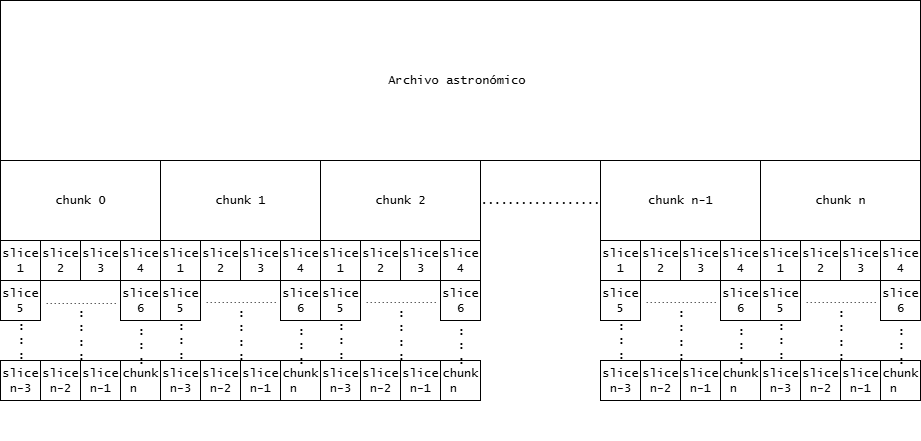
\includegraphics[width=0.9\textwidth]{figures/sistema-chunks.png}
\caption[Esquema de chunks y slices]{Esquema de un archivo astronómico dividido en chunks y slices, ilustrando el concepto de procesamiento con solapamiento. Fuente: Elaboración propia.}
\label{fig:sistema-chunks}
\end{figure}

\subsubsection{Gestión inteligente de memoria y GPU}\label{sec:gpu-memory}

La gestión eficiente de recursos computacionales constituye una mejora fundamental que diferencia DRAFTS++ del prototipo original, el cual carecía de mecanismos sofisticados para la gestión de memoria y recursos GPU. Esta sección define los límites operativos y políticas (presupuestos de RAM/VRAM, limpieza determinística, \textit{fallback} a CPU) que condicionan el plan de \emph{chunk}/\emph{slice} de la Sección \ref{sec:chunk-slice-planning} y el comportamiento en ejecución de la Sección \ref{sec:streaming-continuity}, asegurando estabilidad y rendimiento.

\paragraph{Algoritmo de Planificación de Recursos y Gestión de Memoria Dinámica}

El sistema implementa un \textbf{algoritmo de planificación de recursos} que calcula dinámicamente el tamaño óptimo de \emph{chunks} basándose en la memoria disponible del sistema y las características de los datos. Este algoritmo es fundamental para garantizar que el pipeline pueda procesar observaciones de cualquier tamaño sin desbordamientos de memoria.

El algoritmo de planificación de recursos opera mediante los siguientes pasos:

\begin{enumerate}
    \item \textbf{Cálculo de memoria disponible:} Se determina la memoria RAM disponible del sistema usando \texttt{psutil.virtual\_memory().available}.
    \item \textbf{Estimación de bytes por muestra:} Se calcula el tamaño en bytes que ocupará cada muestra después de la decimación espectral.
    \item \textbf{Aplicación de presupuesto de memoria:} Se reserva un porcentaje de la memoria disponible (típicamente 25\%) para operaciones de \emph{overhead} y estabilidad del sistema.
    \item \textbf{Cálculo de tamaño máximo de chunk:} Se determina el número máximo de muestras que pueden procesarse en un solo \emph{chunk} sin exceder el presupuesto de memoria.
    \item \textbf{Alineación con longitud de slice:} Se ajusta el tamaño del \emph{chunk} para que sea múltiplo exacto de la longitud de \emph{slice}, garantizando contigüidad perfecta.
\end{enumerate}

La formulación matemática del algoritmo se basa en las siguientes ecuaciones, siempre en el dominio temporal ya decimado:

\[
\text{total\_samples}_{\mathrm{ds}} = \left\lfloor \frac{\text{FILE\_LENG}}{\max(1,\text{DOWN\_TIME\_RATE})} \right\rfloor
\]

donde:
\begin{itemize}
    \item $\text{FILE\_LENG}$: Número de muestras crudas del archivo original.
    \item $\text{DOWN\_TIME\_RATE}$: Factor de decimación temporal aplicado.
    \item $\text{total\_samples}_{\mathrm{ds}}$: Muestras resultantes tras la decimación temporal (dominio operativo del pipeline).
\end{itemize}

El peso por muestra decimada depende del número de canales que sobreviven al downsampling en frecuencia:

\[
\text{bytes\_por\_muestra} = 4 \times \left\lfloor \frac{\text{FREQ\_RESO}}{\max(1,\text{DOWN\_FREQ\_RATE})} \right\rfloor
\]

donde:
\begin{itemize}
    \item $\text{FREQ\_RESO}$: Número total de canales de frecuencia originales.
    \item $\text{DOWN\_FREQ\_RATE}$: Factor de decimación espectral aplicado.
    \item El factor $4$: Representa el tamaño en bytes de un valor de punto flotante (32-bit).
\end{itemize}

La fracción de memoria utilizable para chunking queda acotada por la política de presupuesto. Denotando por $\text{memoria\_disponible}$ la memoria RAM libre y por $\text{FRACCION\_MAX\_RAM}$ y $\text{FACTOR\_OVERHEAD}$ los parámetros de configuración (por defecto 0.25 y 1.3 respectivamente), se obtiene:

\[
\text{memoria\_utilizable} = \frac{\text{memoria\_disponible} \times \text{FRACCION\_MAX\_RAM}}{\text{FACTOR\_OVERHEAD}}
\]

Si el archivo ya decimado cabe íntegramente en memoria (condición $\text{total\_samples}_{\mathrm{ds}} \times \text{bytes\_por\_muestra} \le 0.8\,\text{memoria\_disponible}$), se procesa de una sola vez:

\[
\text{chunk\_samples} = \text{total\_samples}_{\mathrm{ds}}
\]

En caso contrario, la política de memoria fija un límite de muestras candidatas

\[
m_{\text{cand}} = \max\!\left(\text{slice\_len},\; \min\!\left(\left\lfloor \frac{\text{memoria\_utilizable}}{\text{bytes\_por\_muestra}} \right\rfloor,\; \text{total\_samples}_{\mathrm{ds}}\right)\right)
\]

y el tamaño final del chunk se alinea a un múltiplo exacto de $\text{slice\_len}$ para preservar la geometría calculada:

\[
\text{chunk\_samples} = \max\!\left(\text{slice\_len},\; \left\lfloor \frac{m_{\text{cand}}}{\text{slice\_len}} \right\rfloor \times \text{slice\_len} \right)
\]

\noindent donde:
\begin{itemize}
    \item $\text{slice\_len}$: Longitud de cada \emph{slice} en muestras decimadas (geometría objetivo calculada en la Sección \ref{sec:chunk-slice-planning}).
    \item $m_{\text{cand}}$: Límite provisional de muestras derivado del presupuesto de memoria y acotado por $\text{total\_samples}_{\mathrm{ds}}$.
    \item $\text{memoria\_utilizable}$: Presupuesto de RAM disponible para un chunk, luego de aplicar los factores $\text{FRACCION\_MAX\_RAM}$ y $\text{FACTOR\_OVERHEAD}$.
    \item $\text{bytes\_por\_muestra}$: Consumo en bytes de una muestra decimada (incluye canales retenidos tras $\text{DOWN\_FREQ\_RATE}$).
    \item $\text{total\_samples}_{\mathrm{ds}}$: Total de muestras temporales disponibles en el dominio decimado del archivo.
\end{itemize}

Este algoritmo garantiza que cada \emph{chunk} sea procesable con la memoria disponible mientras mantiene la eficiencia computacional, preserva la contigüidad temporal y respeta la planificación de \emph{slices}.

\begin{algorithm}[H]
\caption{Planificación de Recursos y Gestión de Memoria Dinámica}
\label{alg:resource-planning}
\begin{algorithmic}[1]
\Require Metadatos del archivo (FREQ\_RESO, DOWN\_FREQ\_RATE, FILE\_LENG)
\Ensure Tamaño óptimo de chunk en muestras

\State \textbf{INICIO}
\State Obtener memoria disponible: $\text{mem\_available} = \text{psutil.virtual\_memory().available}$
\State Calcular canales decimados: $\text{channels\_ds} = \max\!\left(1, \left\lfloor \frac{\text{FREQ\_RESO}}{\max(1,\text{DOWN\_FREQ\_RATE})} \right\rfloor\right)$
\State Calcular bytes por muestra: $\text{bytes\_per\_sample} = 4 \times \text{channels\_ds}$

\If{archivo completo cabe en memoria}
    \State $\text{chunk\_samples} = \text{total\_samples}_{\mathrm{ds}}$
    \State \textbf{RETORNAR} $\text{chunk\_samples}$
\Else
    \State Calcular memoria utilizable: $\text{usable\_mem} = \frac{\text{mem\_available} \times \text{FRACCION\_MAX\_RAM}}{\text{FACTOR\_OVERHEAD}}$
    \State Calcular muestras candidatas: $m_{\text{cand}} = \max\!\left(\text{slice\_len},\; \min\!\left(\left\lfloor \frac{\text{usable\_mem}}{\text{bytes\_per\_sample}} \right\rfloor,\; \text{total\_samples}_{\mathrm{ds}}\right)\right)$
    \State Alinear con slice\_len: $\text{chunk\_samples} = \max\!\left(\text{slice\_len},\; \left\lfloor \frac{m_{\text{cand}}}{\text{slice\_len}} \right\rfloor \times \text{slice\_len} \right)$
\EndIf

\State Validar parámetros calculados
\State \textbf{RETORNAR} $\text{chunk\_samples}$
\State \textbf{FIN}
\end{algorithmic}
\end{algorithm}

\subsubsection{Integración y Automatización del Workflow de Modelos de DRAFTS}

La etapa de procesamiento integrado representa el núcleo computacional más sofisticado del pipeline DRAFTS++, donde se materializa la convergencia entre ingeniería de software avanzada y la integración automatizada de los modelos de deep learning existentes en DRAFTS-main. Esta sección detalla cómo se procesan los datos astronómicos para identificar y clasificar candidatos FRB utilizando los modelos CenterNet y ResNet18 de manera integrada, automatizada y eficiente dentro de un flujo de trabajo unificado.

A diferencia del prototipo DRAFTS-main que ejecutaba los modelos de detección y clasificación como etapas separadas y desacopladas, DRAFTS++ implementa un sistema integrado que automatiza la orquestación de estos modelos, combinando detección de objetos, clasificación binaria y validación científica en un flujo unificado y optimizado. Esta aproximación elimina las limitaciones del procesamiento manual por lotes separado y establece las bases para un sistema productivo capaz de manejar observaciones de larga duración en tiempo real, tal como se conceptualizó originalmente en el workflow de DRAFTS.

El procesamiento integrado opera mediante tres pilares fundamentales: (i) integración automatizada del modelo CenterNet para detección de candidatos FRB, (ii) orquestación en flujo del modelo ResNet18 para clasificación binaria, y (iii) validación física y temporal que asegura la coherencia científica de las detecciones. Esta arquitectura integrada representa una mejora significativa sobre el prototipo original, que carecía de integración coherente entre estas etapas y requería intervención manual para coordinar los modelos.

\begin{figure}[H]
\centering
\resizebox{\textwidth}{!}{%
\begin{tikzpicture}[
    node distance=0.8cm and 1.4cm,
    stage/.style={rectangle, draw, fill=blue!20, text width=2.0cm, text centered, minimum height=0.7cm, font=\scriptsize},
    model/.style={rectangle, draw, fill=green!20, text width=1.8cm, text centered, minimum height=0.6cm, font=\scriptsize},
    validation/.style={rectangle, draw, fill=orange!20, text width=1.8cm, text centered, minimum height=0.6cm, font=\scriptsize},
    arrow/.style={-Stealth, thick},
    dataflow/.style={-Stealth, thick, dashed, blue}
]

% Entrada
\node[stage] (input) {Imagen\\DM-tiempo};

% CenterNet
\node[model, right=of input] (centernet) {CenterNet\\Detección};

% ResNet18
\node[model, right=of centernet] (resnet) {ResNet18\\Clasificación};

% Validación
\node[validation, right=of resnet] (validation) {Validación\\Física/Temporal};

% Salida
\node[stage, right=of validation] (output) {Candidatos\\Validados};

% Flujo principal
\draw[arrow] (input) -- (centernet);
\draw[arrow] (centernet) -- (resnet);
\draw[arrow] (resnet) -- (validation);
\draw[arrow] (validation) -- (output);

% Etiquetas de datos
\node[above=0.2cm of centernet] {\tiny Candidatos $(DM, t, box)$};
\node[above=0.2cm of resnet] {\tiny Probabilidad $p$};
\node[above=0.2cm of validation] {\tiny Métricas SNR, $t_{abs}$};

\end{tikzpicture}%
}
\caption[Workflow integrado DRAFTS++]{Workflow integrado y automatizado de DRAFTS++: procesamiento secuencial desde detección con CenterNet, clasificación con ResNet18, hasta validación física y temporal, eliminando la necesidad de procesamiento manual por lotes separado del prototipo original.}
\label{fig:integrated-workflow}
\end{figure}
\paragraph{Integración Automatizada del Modelo CenterNet}

El sistema de detección integra el modelo CenterNet existente en DRAFTS-main, una arquitectura de deep learning especializada en detección de objetos, que fue previamente entrenada para identificar candidatos FRB en imágenes DM-tiempo. La contribución de DRAFTS++ no radica en el desarrollo o entrenamiento de este modelo, sino en la implementación de la infraestructura de software necesaria para embeber, ejecutar y orquestar este modelo de manera automatizada dentro del pipeline de streaming.

CenterNet opera mediante la detección de objetos como puntos centrales en el espacio de la imagen, eliminando la necesidad de anclas y procesos de supresión no máxima (NMS). Esta aproximación es particularmente efectiva para detectar transientes rápidos como FRBs, donde la forma y localización precisa son críticas para la validación científica posterior. DRAFTS++ proporciona la infraestructura de software para ejecutar este modelo de manera eficiente y automática.

El algoritmo de integración y ejecución de CenterNet en DRAFTS++ se implementa mediante los siguientes pasos:

\begin{enumerate}
    \item \textbf{Preprocesamiento de imagen:} La imagen DM-tiempo se normaliza y redimensiona a 512×512 píxeles, aplicando normalización estadística y corrección de color para optimizar la entrada del modelo pre-entrenado.
    \item \textbf{Carga y ejecución del modelo:} Se carga el modelo CenterNet pre-entrenado desde los checkpoints existentes en DRAFTS-main y se ejecuta la inferencia sobre la imagen preprocesada.
    \item \textbf{Procesamiento de salidas:} El modelo genera tres mapas de salida: mapa de calor $H$ (centros de objetos), regresión de tamaño $WH$ (dimensiones), y regresión de desplazamiento $OFF$ (correcciones de posición).
    \item \textbf{Post-procesamiento y extracción de candidatos:} Se aplica supresión no máxima adaptada y filtrado por confianza para generar las detecciones finales, extrayendo coordenadas DM-tiempo de los candidatos detectados.
\end{enumerate}

La formulación matemática del modelo CenterNet se basa en las siguientes ecuaciones:

El mapa de calor se genera mediante:

\[
H_{x,y} = \sigma\left(\sum_{i=1}^{N} \exp\left(-\frac{(x - x_i)^2 + (y - y_i)^2}{2\sigma^2}\right)\right)
\]

donde:
\begin{itemize}
    \item $H_{x,y}$: Valor del mapa de calor en la posición $(x,y)$
    \item $N$: Número de objetos en la imagen
    \item $(x_i, y_i)$: Posición central del objeto $i$
    \item $\sigma$: Parámetro de dispersión gaussiana (típicamente 2.0)
    \item $\sigma(\cdot)$: Función de activación sigmoide
\end{itemize}

La regresión de tamaño predice las dimensiones del objeto mediante:

\[
(w, h) = f_{wh}(F_{x_c, y_c})
\]

donde $f_{wh}$ es una función aprendida que mapea las características locales $F_{x_c, y_c}$ a las dimensiones del objeto.

La regresión de desplazamiento calcula la corrección de posición:

\[
(\Delta x, \Delta y) = f_{off}(F_{x_c, y_c})
\]

donde $f_{off}$ predice el desplazamiento respecto al centro del píxel más cercano.

\begin{algorithm}[H]
\caption{Detección de Candidatos FRB con CenterNet}
\label{alg:centernet-detection}
\begin{algorithmic}[1]
\Require Imagen DM-tiempo $I$, modelo CenterNet entrenado
\Ensure Lista de candidatos con coordenadas y confianza

\State \textbf{INICIO}
\State Normalizar imagen: $I_{norm} = \text{normalize}(I)$
\State Redimensionar a 512×512: $I_{resized} = \text{resize}(I_{norm})$
\State Convertir a tensor: $T = \text{to\_tensor}(I_{resized})$

\State \textbf{Inferencia del modelo}
\State $H, WH, OFF = \text{model}(T)$ \Comment{Mapas de calor, tamaño y desplazamiento}
\State Aplicar sigmoide al mapa de calor: $H = \sigma(H)$

\State \textbf{Post-procesamiento}
\State Extraer picos locales: $\text{peaks} = \text{find\_peaks}(H, \text{threshold}=\theta)$
\For{cada pico $p$ en peaks}
    \State $(x_c, y_c) = \text{coordenadas}(p)$
    \State $(w, h) = WH[x_c, y_c]$ \Comment{Regresión de tamaño}
    \State $(\Delta x, \Delta y) = OFF[x_c, y_c]$ \Comment{Regresión de desplazamiento}
    \State Calcular caja delimitadora: $box = [x_c + \Delta x - w/2, y_c + \Delta y - h/2, x_c + \Delta x + w/2, y_c + \Delta y + h/2]$
    \State Calcular DM y tiempo: $(DM, t) = \text{convert\_to\_physical}(box)$
    \State Agregar candidato: $\text{candidates.append}(DM, t, \text{confidence}(p))$
        \EndFor

\State \textbf{RETORNAR} candidates
\State \textbf{FIN}
\end{algorithmic}
\end{algorithm}
\paragraph{Orquestación Automatizada del Modelo ResNet18}

El sistema de clasificación integra el modelo ResNet18 existente en DRAFTS-main, una arquitectura de red neuronal residual previamente entrenada para clasificación binaria de FRBs, que opera en tiempo real durante el procesamiento, evaluando cada candidato detectado por CenterNet para determinar si representa un FRB genuino o ruido. La contribución de DRAFTS++ radica en la automatización de la orquestación entre los modelos, eliminando la necesidad de procesamiento manual por lotes separado.

La clasificación binaria se basa en la extracción de características de patches dedispersados correspondientes a cada candidato detectado por CenterNet. El modelo ResNet18 utiliza una arquitectura residual previamente entrenada para procesar imágenes de FRBs, específicamente diseñada para distinguir entre transientes genuinos y artefactos instrumentales. DRAFTS++ proporciona la infraestructura de software para ejecutar este modelo de manera automatizada y en flujo continuo.

El algoritmo de orquestación y ejecución de ResNet18 en DRAFTS++ opera mediante los siguientes pasos:

\begin{enumerate}
    \item \textbf{Extracción de patch:} Se extrae una región de interés (ROI) alrededor de cada candidato detectado por CenterNet en la imagen DM-tiempo.
    \item \textbf{Dedispersión:} Se aplica dedispersión al patch utilizando el DM detectado para obtener la señal temporal integrada.
    \item \textbf{Preprocesamiento:} Se normaliza el patch dedispersado aplicando corrección de tendencia y normalización estadística para optimizar la entrada del modelo pre-entrenado.
    \item \textbf{Carga y ejecución del modelo:} Se carga el modelo ResNet18 pre-entrenado desde los checkpoints existentes en DRAFTS-main y se ejecuta la inferencia sobre el patch preprocesado.
    \item \textbf{Interpretación de probabilidades:} Se interpreta la salida del modelo para obtener la probabilidad intrínseca de pertenencia a la clase FRB, tal como se visualiza en el workflow original de DRAFTS.
    \item \textbf{Decisión automatizada:} Se aplica un umbral de confianza configurable para clasificar automáticamente el candidato como "BURST" o "NO BURST".
\end{enumerate}

La formulación matemática del proceso de clasificación se basa en las transformaciones exactas implementadas en el módulo 	exttt{model	extunderscore interface}. El preprocesamiento del patch sigue cuatro pasos determinísticos:

\[
P^{(1)} = P + \mathbf{1}, \qquad
P^{(2)}_{i,j} = \frac{P^{(1)}_{i,j}}{\mu_j}, \qquad
P^{(3)} = \operatorname{clip}\big(P^{(2)}, q_{5}, q_{95}\big),
\]

\[
P_{\text{final}} = \frac{P^{(3)} - \min P^{(3)}}{\max P^{(3)} - \min P^{(3)}}
\]

donde:
\begin{itemize}
    \item $P$: Patch dedispersado original (tiempo \texttimes{} frecuencia).
    \item $\mathbf{1}$: Matriz de unos con la misma forma que $P$, que desplaza la señal para evitar valores nulos.
    \item $\mu_j = \frac{1}{N_t} \sum_i P^{(1)}_{i,j}$: Media de la columna $j$ (normalización por canal de frecuencia).
    \item $q_{5}$ y $q_{95}$: Percentiles 5$^{\circ}$ y 95$^{\circ}$ calculados sobre todos los elementos de $P^{(2)}$.
    \item $\operatorname{clip}(\cdot)$: Operador que limita cada valor al rango $[q_{5}, q_{95}]$ para mitigar outliers.
    \item $\min P^{(3)}$ y $\max P^{(3)}$: Valores mínimo y máximo globales de $P^{(3)}$, usados para el escalado min--max final.
\end{itemize}

La probabilidad de clasificación se calcula mediante:

\[
p = \sigma(W \cdot \phi(P_{final}) + b)
\]

donde:
\begin{itemize}
    \item $p$: Probabilidad de pertenencia a la clase FRB
    \item $\sigma$: Función de activación sigmoide
    \item $W, b$: Pesos y sesgo de la capa de clasificación
    \item $\phi(P_{final})$: Características extraídas por la red convolucional
\end{itemize}

La decisión de clasificación se realiza mediante:

\[
\text{Clase} = \begin{cases} 
\text{BURST} & \text{si } p \geq \theta_{class} \\
\text{NO BURST} & \text{si } p < \theta_{class}
\end{cases}
\]

donde $\theta_{class}$ es el umbral de confianza configurable (típicamente 0.6).

\begin{algorithm}[H]
\caption{Clasificación Binaria en Flujo}
\label{alg:binary-classification}
\begin{algorithmic}[1]
\Require Candidato $(DM, t, box)$, modelo clasificador, datos originales
\Ensure Probabilidad de FRB y clasificación final

\State \textbf{INICIO}
\State Extraer patch de la imagen DM-tiempo: $P = \text{extract\_patch}(box)$
\State Aplicar dedispersión: $P_{dedisp} = \text{dedisperse}(P, DM)$
\State Normalizar patch: $P_{norm} = \frac{P_{dedisp} - \mu}{\sigma} \cdot \frac{1}{\text{mean}(P_{dedisp})} + 1$
\State Aplicar clipping: $v_{min}, v_{max} = \text{percentiles}(P_{norm}, [5, 95])$
\State Normalización final: $P_{final} = \frac{\text{clip}(P_{norm}, v_{min}, v_{max}) - v_{min}}{v_{max} - v_{min}}$

\State \textbf{Clasificación}
\State Convertir a tensor: $T = \text{to\_tensor}(P_{final}[None, None, :, :])$
\State Inferencia: $logits = \text{classifier\_model}(T)$
\State Calcular probabilidad: $p = \text{softmax}(logits)[0, 1]$

\If{$p \geq \theta_{class}$}
    \State $\text{clase} = \text{BURST}$
\Else
    \State $\text{clase} = \text{NO BURST}$
\EndIf

\State \textbf{RETORNAR} $(p, \text{clase})$
\State \textbf{FIN}
\end{algorithmic}
\end{algorithm}
\paragraph{Validación Física y Temporal Integrada}

El sistema de validación implementa verificaciones científicas robustas que aseguran la coherencia física y temporal de los candidatos detectados. Esta validación integrada representa una mejora fundamental sobre el prototipo original, que carecía de verificaciones sistemáticas de calidad.

La validación física se basa en el cálculo de métricas SNR (Signal-to-Noise Ratio) utilizando técnicas de análisis espectral robustas. Se implementa un algoritmo de detección de picos basado en filtrado adaptado que identifica señales significativas en el ruido de fondo.

La validación temporal garantiza la precisión en la localización temporal de los eventos, calculando timestamps absolutos con correcciones por chunk, slice y offset de muestreo. Esta precisión temporal es crucial para la validación científica posterior y la correlación con observaciones independientes.

El algoritmo de validación opera mediante los siguientes pasos:

\begin{enumerate}
    \item \textbf{Cálculo de SNR:} Se calcula el SNR del candidato en la región detectada y en el patch dedispersado.
    \item \textbf{Validación de DM:} Se verifica que el DM detectado esté dentro de rangos físicamente plausibles.
    \item \textbf{Cálculo de tiempo absoluto:} Se calcula el timestamp absoluto con correcciones por chunk y slice.
    \item \textbf{Validación de anchura:} Se estima la anchura temporal del pulso mediante análisis espectral.
    \item \textbf{Validación de coherencia:} Se verifica la consistencia entre las métricas calculadas.
\end{enumerate}

La formulación matemática del cálculo de SNR se basa en:

El SNR se calcula mediante análisis espectral PRESTO-style:

\[
\text{SNR} = \max_w \frac{\text{conv}(s, \text{boxcar}(w))}{\sqrt{w}}
\]

donde:
\begin{itemize}
    \item $s$: Serie temporal dedispersada
    \item $\text{boxcar}(w)$: Kernel de convolución de anchura $w$
    \item $\text{conv}(\cdot, \cdot)$: Operación de convolución
    \item El máximo se toma sobre anchuras $w \in \{1, 2, 3, 4, 6, 9, 14, 20, 30\}$
\end{itemize}

El cálculo de tiempo absoluto se realiza mediante:

\[
t_{abs} = t_{chunk} + t_{slice} + t_{offset} + t_{peak}
\]

donde:
\begin{itemize}
    \item $t_{chunk}$: Tiempo de inicio del chunk
    \item $t_{slice}$: Offset temporal del slice dentro del chunk
    \item $t_{offset}$: Offset de muestreo dentro del slice
    \item $t_{peak}$: Posición del pico dentro del patch dedispersado
\end{itemize}

La validación de DM se realiza mediante:

\[
\text{DM}_{valid} = \begin{cases} 
\text{True} & \text{si } 0 < \text{DM} < \text{DM}_{max} \\
\text{False} & \text{en otro caso}
\end{cases}
\]

donde $\text{DM}_{max}$ es el máximo DM físicamente plausible (típicamente 2000 pc/cm³).

\begin{algorithm}[H]
\caption{Validación Física y Temporal Integrada}
\label{alg:physical-temporal-validation}
\begin{algorithmic}[1]
\Require Candidato $(DM, t, box)$, patch dedispersado, metadatos temporales
\Ensure Métricas de validación y flag de aceptación

\State \textbf{INICIO}
\State Calcular SNR en región candidata: $\text{SNR}_{raw} = \text{compute\_snr}(box)$
\State Calcular SNR en patch dedispersado: $\text{SNR}_{dedisp} = \text{compute\_snr}(patch)$
\State Validar DM: $\text{DM}_{valid} = (0 < DM < 2000)$

\State \textbf{Cálculo de tiempo absoluto}
\State $t_{chunk} = \text{chunk\_start\_sample} \times \text{TIME\_RESO}$
\State $t_{slice} = \text{slice\_start\_idx} \times \text{TIME\_RESO} \times \text{DOWN\_TIME\_RATE}$
\State $t_{offset} = t \times \text{TIME\_RESO} \times \text{DOWN\_TIME\_RATE}$
\State $t_{peak} = \text{peak\_idx} \times \text{TIME\_RESO} \times \text{DOWN\_TIME\_RATE}$
\State $t_{abs} = t_{chunk} + t_{slice} + t_{offset} + t_{peak}$

\State \textbf{Estimación de anchura}
\State $width\_profile = \text{compute\_width\_profile}(patch)$
\State $width\_ms = \text{width\_profile}[\text{peak\_idx}] \times \text{TIME\_RESO} \times \text{DOWN\_TIME\_RATE} \times 1000$

\State \textbf{Validación de coherencia}
\If{$\text{SNR}_{dedisp} \geq \text{SNR}_{threshold}$ y $\text{DM}_{valid}$ y $width\_ms > 0$}
    \State $\text{validated} = \text{True}$
\Else
    \State $\text{validated} = \text{False}$
\EndIf

\State \textbf{RETORNAR} $(\text{SNR}_{raw}, \text{SNR}_{dedisp}, t_{abs}, width\_ms, \text{validated})$
\State \textbf{FIN}
\end{algorithmic}
\end{algorithm}

Esta implementación integrada de detección, clasificación y validación representa una mejora arquitectónica fundamental que establece las bases para un sistema productivo robusto, capaz de procesar observaciones de larga duración con precisión científica y eficiencia computacional optimizada. La contribución clave de DRAFTS++ radica en la automatización y orquestación de los modelos existentes de DRAFTS, transformando un workflow conceptual en un sistema operativo que funciona tal como se visualizó originalmente en el diseño de DRAFTS, con detección y clasificación automatizadas y probabilidades intrínsecas integradas en el flujo de trabajo.


% =============================================================
% Bloque 2: Sólo títulos y subtítulos (estructura)
% =============================================================
\subsection{Bloque 2: Extensión a Alta Frecuencia - Cuatro Líneas de Investigación}

Este bloque explora estrategias metodológicas para extender las capacidades de detección hacia regímenes de alta frecuencia (30-100 GHz), donde las firmas dispersivas tradicionales se atenúan significativamente. La detección de FRBs en el régimen milimétrico presenta desafíos fundamentales que requieren aproximaciones metodológicas diferenciadas.

A estas frecuencias, la dispersión temporal se atenúa significativamente debido a la dependencia cuadrática inversa con la frecuencia, resultando en firmas dispersivas que pueden ser indistinguibles del ruido instrumental en resoluciones temporales típicas. Este bloque presenta cuatro líneas de investigación complementarias que abordan diferentes aspectos del desafío de detección en el espectro milimétrico.

\subsubsection{Línea 1: Validación de DRAFTS++ sin modificaciones}

Esta línea constituye una extensión natural del Bloque 1: se emplea \textbf{exactamente el mismo DRAFTS++ sin modificaciones}, preservando la arquitectura y el \emph{workflow} clásico (DM-tiempo para propuesta y red de clasificación para decisión), con el propósito de \textit{medir su capacidad base} en regímenes de alta frecuencia. El interés es doble: (i) establecer la sensibilidad y robustez mínima alcanzable sin introducir nuevas heurísticas ni rutas alternativas, y (ii) cuantificar objetivamente el punto a partir del cual las estrategias específicas de alta frecuencia (Línea 2) superan al flujo original en eficacia operativa. El criterio físico de resolubilidad se expresa mediante el retardo dispersivo máximo entre los extremos de banda,
\[
\Delta t_{\mathrm{ms}} = 4.148808 \times 10^{3}\,\, \mathrm{DM}\,\big(\nu_{\mathrm{low}}^{-2}-\nu_{\mathrm{high}}^{-2}\big),
\]

\noindent donde:
\begin{itemize}
    \item $\Delta t_{\mathrm{ms}}$: retardo dispersivo entre los extremos de banda, en milisegundos.
    \item $\mathrm{DM}$: medida de dispersión de la línea de visión, en pc\,cm$^{-3}$.
    \item $\nu_{\mathrm{low}}, \, \nu_{\mathrm{high}}$: frecuencias de borde inferior y superior de la banda, en GHz.
    \item $t_{\mathrm{samp}}$: resolución temporal efectiva de muestreo del dato, en ms.
    \item $\alpha$: factor de seguridad adimensional usado en el criterio de resolubilidad (típicamente 1.5--2.0).
\end{itemize}
comparado con la resolución temporal efectiva $t_{\mathrm{samp}}$. Cuando $\Delta t_{\mathrm{ms}} > \alpha\, t_{\mathrm{samp}}$ (con $\alpha$ de seguridad en el rango 1.5–2.0), el \textit{bow–tie} permanece resoluble y la detección en DM-tiempo sigue siendo pertinente; si $\Delta t_{\mathrm{ms}} \le \alpha\, t_{\mathrm{samp}}$, la firma se comprime y el mapa DM-tiempo pierde contraste, anticipándose una disminución de sensibilidad. La validación consiste, por tanto, en aplicar el flujo sin modificaciones sobre ventanas en las que $\Delta t_{\mathrm{ms}}$ sea resoluble y medir sensibilidad, tasa de falsos positivos y estabilidad temporal del detector; este resultado sirve de referencia objetiva para las estrategias alternativas descritas a continuación.


\subsubsection{Línea 2: Detección por SNR con clasificación binaria en flujo}

Cuando el retardo dispersivo se vuelve comparable o inferior a la resolución temporal, el patrón DM-tiempo pierde contraste y la representación más informativa pasa a ser el perfil temporal. Inspirada en el enfoque clásico de \textbf{PRESTO} \cite{2011ascl.soft07017R}, esta línea introduce una \textbf{rama SNR-threshold} dentro del \emph{workflow} original de DRAFTS++: la \textit{propuesta} deja de realizarse con un detector en DM–tiempo y pasa a ejecutarse con un umbral de SNR en la serie temporal; la \textit{decisión} final se mantiene en la red de clasificación binaria ya integrada. Arquitectónicamente, la rama se \textit{activa condicionalmente} cuando el módulo de análisis determina que $\Delta t_{\mathrm{ms}} \le \alpha\, t_{\mathrm{samp}}$ (pérdida de \textit{bow–tie}). Tras proponer con SNR, el flujo \textit{regresa} a la ruta estándar: dedispersión local coherente, clasificación binaria, validaciones físicas y emisión de artefactos estandarizados. Este diseño es atractivo porque (i) conserva el carácter E2E y la unificación de salidas, (ii) reduce el costo de exploración en dominios con poca separabilidad DM-tiempo, y (iii) reutiliza la misma infraestructura de clasificación, auditoría y trazabilidad.

Sea $s(t)$ la serie temporal (obtenida por integración en frecuencia y normalización robusta). La estimación de SNR por filtrado adaptado se define como
\[
\mathrm{SNR}(t) = \max_{w\in\mathcal{W}} \frac{\big(s * b_w\big)(t)}{\sqrt{w}},
\]
\noindent donde:
\begin{itemize}
    \item $s(t)$: serie temporal integrada en frecuencia y normalizada robustamente.
    \item $b_w$: función \textit{boxcar} de anchura temporal $w$.
    \item $\mathcal{W}$: conjunto discreto de anchos de \textit{boxcar} para filtrado adaptado.
    \item $\mathrm{SNR}(t)$: relación señal-ruido estimada en el instante $t$.
    \item $T$: umbral de detección SNR (típicamente 6-10).
    \item $t_i$: instantes candidatos que superan el umbral SNR.
    \item $\Delta t_{\min}$: separación temporal mínima entre candidatos para evitar duplicidades.
    \item $\mathrm{DM}^*$: medida de dispersión óptima local estimada por maximización de coherencia temporal.

La detección primaria consiste en seleccionar instantes $t_i$ tales que $\mathrm{SNR}(t_i)\ge T$ y $|t_i-t_j|\ge \Delta t_{\min}$ para todo $j\ne i$, lo que evita duplicidades y reagregaciones espurias. Alrededor de cada $t_i$ se construye un parche tiempo-frecuencia centrado en $t_i$ y se evalúa una rejilla local de medidas de dispersión para obtener $\mathrm{DM}^*$ como el valor que maximiza la coherencia temporal dedispersada. Este parche, dedispersado a $\mathrm{DM}^*$ y preprocesado, se somete a la red de clasificación binaria para estimar la probabilidad intrínseca de pertenencia a la clase FRB. Finalmente, se exige consistencia física mínima (por ejemplo, $\mathrm{DM}^*>0$ con incertidumbre acotada y anchura temporal finita) antes de emitir el candidato.

\end{itemize}

\begin{algorithm}[H]
\caption{Detección híbrida HF: SNR $\rightarrow$ parche dedispersado $\rightarrow$ clasificación}
\label{alg:hf-snr-class}
\begin{algorithmic}[1]
\Require Serie temporal $s(t)$, umbral $T$, separación $\Delta t_{\min}$, conjunto de anchos $\mathcal{W}$, rejilla local de DM
\Ensure Candidatos validados con $\{t_{\mathrm{evt}},\, \mathrm{SNR},\, \mathrm{DM}^*,\, p\}$

\State Normalizar $s(t)$ de forma robusta (tendencia y escala)
\State Calcular $\mathrm{SNR}(t)=\max_{w\in\mathcal{W}} (s*b_w)(t)/\sqrt{w}$
\State Extraer picos $\{t_i\}$ con $\mathrm{SNR}(t_i)\ge T$ y distancia mínima $\Delta t_{\min}$
\For{cada $t_i$}
    \State Construir un parche tiempo–frecuencia centrado en $t_i$
    \State Evaluar la rejilla local de DM y obtener $\mathrm{DM}^*$ por máxima coherencia
    \State Dedispersar y preprocesar el parche a $\mathrm{DM}^*$
    \State Estimar probabilidad binaria $p$ con el clasificador en flujo
    \If{$p$ suficientemente alto y $\mathrm{DM}^*>0$ con anchura temporal finita}
        \State Emitir candidato con $(t_{\mathrm{evt}}\!=\!t_i,\, \mathrm{SNR}(t_i),\, \mathrm{DM}^*,\, p)$
    \EndIf
\EndFor
\end{algorithmic}
\end{algorithm}

\begin{figure}[H]
\centering
\resizebox{\textwidth}{!}{%
\begin{tikzpicture}[
    node distance=0.9cm and 1.6cm,
    stage/.style={rectangle, draw, fill=blue!20, text width=2.3cm, text centered, minimum height=0.7cm, font=\scriptsize},
    decision/.style={diamond, draw, fill=yellow!20, aspect=2, text width=2.4cm, text centered, inner sep=1pt, font=\scriptsize},
    arrow/.style={-Stealth, thick}
]

% Nodos principales
\node[stage] (input) {Archivo\\HF};
\node[decision, right=of input] (cond) {$\Delta t_{\mathrm{ms}} > \alpha\,t_{\mathrm{samp}}$?};
\node[stage, below right=of cond] (snr) {Propuesta por SNR};
\node[stage, above right=of cond] (dmmap) {Propuesta DM--tiempo};
\node[stage, right=3.0cm of snr] (dedisp) {Dedispersión local};
\node[stage, right=of dedisp] (clf) {Clasificación Binaria};
\node[stage, right=of clf] (val) {Validación Física};
\node[stage, right=of val] (out) {Artefactos\\Estandarizados};

% Flujo
\draw[arrow] (input) -- (cond);
\draw[arrow] (cond) -- node[above] {Sí} (dmmap);
\draw[arrow] (cond) -- node[below] {No} (snr);
\draw[arrow] (snr) -- (dedisp);
\draw[arrow] (dmmap) |- (dedisp);
\draw[arrow] (dedisp) -- (clf);
\draw[arrow] (clf) -- (val);
\draw[arrow] (val) -- (out);

\end{tikzpicture}}
\caption[Rama SNR en el workflow HF]{Rama SNR-threshold para alta frecuencia integrada en el workflow de DRAFTS++: la condición física activa la propuesta por SNR cuando el \textit{bow–tie} no es resoluble; el flujo vuelve a la ruta estándar para dedispersión local, clasificación y validación.}
\label{fig:hf-snr-branch}
\end{figure}

\subsubsection{Línea 3: Nuevos Plots Característicos}

En frecuencias milimétricas, la ausencia de la firma dispersiva clásica (``bow-tie'') elimina el principal discriminador visual entre señales astrofísicas genuinas e interferencia de radiofrecuencia. Esta pérdida de información morfológica requiere la exploración de representaciones 2D alternativas que capturen características distintivas de pulsos cósmicos en regímenes donde $\Delta t_{\mathrm{ms}} \ll t_{\mathrm{samp}}$. Las siguientes propuestas de \textit{plots} característicos buscan ``engañar'' a las redes neuronales de detección mediante la generación artificial de patrones visuales que permitan la identificación de FRBs a pesar de la compresión dispersiva.

\paragraph{Estado de Desarrollo}

La implementación de las representaciones 2D alternativas se encuentra actualmente en desarrollo activo en una rama separada del repositorio de DRAFTS++ en GitHub. Esta línea de investigación está aislada del pipeline principal para permitir experimentación y refinamiento independiente sin comprometer la estabilidad del sistema productivo. La integración en el pipeline unificado se realizará una vez que las implementaciones alcancen un estado de madurez suficiente para su validación experimental completa.

\paragraph{Espectrograma Dinámico Polarimétrico (Tiempo–Frecuencia con Stokes IQUV)}

Una representación fundamental consiste en enriquecer el espectrograma tradicional con información polarimétrica completa. En lugar de usar únicamente la intensidad total (Stokes I), se construye una imagen multicanal que incluye los cuatro parámetros de Stokes I, Q, U, V como capas superpuestas. Cada píxel $(t,f)$ contiene un vector de 4 valores que puede procesarse como imagen RGB con canal adicional por una CNN. Esta representación aprovecha el hecho de que los FRBs exhiben típicamente polarización extrema (>50\%), mientras que la RFI terrestre tiende a ser no polarizada o con polarización constante.

Un FRB altamente polarizado aparecerá como una traza vertical simultánea en el canal I (intensidad) y en los canales Q/U (polarización lineal), generando una ``firma'' multicanal coherente. La rotación Faraday, aunque reducida en mm, aún puede manifestarse como variaciones sistemáticas en Q/U a través de la banda, creando patrones de ``ondulación'' que las CNNs pueden aprender a reconocer como características de origen astrofísico.

\paragraph{Mapa Tiempo-Ancho de Pulso (Multi-Escala Temporal)}

Esta representación explora la respuesta de la señal a diferentes filtros de integración temporal. El eje horizontal representa el tiempo, mientras que el eje vertical codifica el ancho de ventana de integración aplicado. Para cada tiempo $t$ y ancho $w$, se calcula la SNR de la señal integrada en una ventana $\pm w/2$ alrededor de $t$.

Un pulso astrofísico genuino de duración intrínseca $\tau$ produce un patrón característico tipo ``triángulo invertido'': máxima SNR en la fila correspondiente a $w \approx \tau$, con atenuación gradual para anchos mayores (dilución en ruido) y menores (no capturan toda la energía). Esta morfología multi-escala es distintiva de pulsos cósmicos, ya que la RFI tiende a ser o extremadamente breve (una sola muestra) o persistentemente extendida, generando patrones fundamentalmente diferentes.

La ventaja de esta representación radica en su capacidad de ``simular'' la estructura temporal que la dispersión proporciona en frecuencias bajas, creando artificialmente una dimensión discriminativa donde los FRBs muestran concentración de energía en escalas específicas, mientras que la RFI aparece distribuida o ausente de picos definidos.

\paragraph{Mapa Tiempo-RM (Rotación Faraday versus Tiempo)}

Para datos polarimétricos, se puede construir un mapa que explore el espacio de rotación Faraday. Similar a como la dispersión DM introduce retardos en frecuencia, la RM introduce giros en la polarización lineal. Para cada instante temporal, se evalúa cómo varía la potencia polarizada al asumir diferentes valores de RM mediante rotación de los vectores Q/U.

Un pulso astrofísico altamente polarizado produce una franja vertical brillante en el mapa tiempo–RM, alineada con su RM verdadera. En contraste, la RFI terrestre raramente presenta rotación Faraday significativa, apareciendo principalmente cerca de RM = 0. Esta representación ``engaña'' a la red neuronal al proporcionar una dimensión adicional de discriminación: la capacidad de distinguir pulsos con RM elevados (típicos de entornos magnetizados cósmicos) de interferencia local.

\paragraph{Mapa de Coherencia Espectral (Correlación en Frecuencia)}

Esta representación menos convencional captura la extensión en frecuencia de una señal mediante autocorrelación espectral. Para cada intervalo temporal, se calcula la autocorrelación del vector de intensidades por frecuencia, midiendo cuán ancha en espectro es la señal.

Los pulsos astrofísicos, siendo típicamente broadband, producen autocorrelaciones que persisten hasta lags de frecuencia grandes, manifestándose como franjas horizontales extendidas en el mapa tiempo–lag. Por el contrario, la RFI narrowband genera correlaciones que decaen abruptamente, apareciendo como líneas delgadas confinadas a lag $\approx$ 0. Esta representación ``simula'' la coherencia espectral que caracteriza a los pulsos cósmicos, proporcionando a la CNN un criterio adicional para distinguir emisiones de banda ancha genuinas de interferencia localizada.

\paragraph{Estrategia de ``Bow-tie Artificial'' mediante Combinación de Representaciones}

La propuesta más innovadora consiste en combinar múltiples representaciones para generar artificialmente una ``firma bow-tie'' en el espacio de características de alta dimensión. Mediante la concatenación de los mapas tiempo–ancho, tiempo–RM, y coherencia espectral, se crea una imagen multicanal donde cada representación aporta una ``dimensión'' del patrón dispersivo perdido:

\[
\mathbf{I}_{\mathrm{combined}} = \mathrm{concat}[\mathbf{I}_{\mathrm{width}}, \mathbf{I}_{\mathrm{RM}}, \mathbf{I}_{\mathrm{coherence}}]
\]

donde $\mathbf{I}_{\mathrm{width}}$, $\mathbf{I}_{\mathrm{RM}}$, y $\mathbf{I}_{\mathrm{coherence}}$ representan las representaciones 2D correspondientes. Un FRB genuino manifestará patrones coherentes en todas las dimensiones: pico temporal en tiempo–ancho, alineación polarimétrica en tiempo–RM, y persistencia espectral en coherencia, generando una ``firma multidimensional'' que la CNN puede aprender a reconocer como equivalente al bow-tie dispersivo clásico.

Esta estrategia de ``engaño neuronal'' preserva la filosofía DM-centrada de DRAFTS mientras adapta la detección a regímenes donde la dispersión temporal es despreciable, manteniendo la capacidad discriminativa mediante representaciones alternativas que capturan aspectos fundamentales de la física de pulsos astrofísicos.

\subsubsection{Línea 4: Estrategias Alternativas del Autor de DRAFTS}

En respuesta a los desafíos específicos de detección de FRBs en frecuencias milimétricas, \textbf{Yong-Kun Zhang}, autor original de DRAFTS, ha propuesto dos estrategias complementarias para abordar la atenuación del retardo dispersivo en regímenes de alta frecuencia. Estas propuestas surgen directamente de la limitación fundamental del paradigma DM-centrado: cuando $\Delta t_{\mathrm{ms}} \ll t_{\mathrm{samp}}$, la firma dispersiva \textit{bow-tie} se comprime hasta volverse indistinguible del ruido, eliminando la capacidad discriminativa principal entre señales astrofísicas genuinas e interferencia de radiofrecuencia (RFI).

\paragraph{Estado de Desarrollo}

Las estrategias alternativas de Zhang se encuentran actualmente en implementación en una rama dedicada del repositorio de DRAFTS++ en GitHub. Esta línea de investigación está siendo desarrollada de forma aislada para permitir experimentación extensiva con los algoritmos de expansión de rejilla DM y validación DM-aware, sin afectar la estabilidad del pipeline principal. La integración completa en el sistema unificado se realizará tras la validación experimental de estas estrategias avanzadas.

La \textbf{Estrategia 1} propuesta por Zhang consiste en \textit{expandir el rango y granularidad de DM} mediante una exploración sistemática del plano tiempo-DM con parámetros adaptados a la compresión dispersiva. En lugar de mantener las rejillas DM estándar optimizadas para frecuencias bajas, se implementa un barrido con rangos ampliados y pasos más gruesos, forzando artificialmente la ``apertura'' de pulsos reales en formas \textit{bow-tie} detectables. Matemáticamente, esto se expresa como una transformación de la rejilla DM tradicional:

\[
\mathcal{D}_{\mathrm{traditional}} = \{d_i : d_i = d_{\min} + i \cdot \delta d, \; i \in [0, N_{\mathrm{DM}}]\}
\]

\[
\mathcal{D}_{\mathrm{expanded}} = \{d_j : d_j = d_{\min} + j \cdot \gamma \delta d, \; j \in [0, \lfloor N_{\mathrm{DM}}/\gamma \rfloor]\}
\]

donde $\gamma > 1$ es el factor de expansión del paso DM y $d_{\min}$ se extiende a valores más bajos para capturar señales de baja dispersión. La detección se realiza mediante la condición de que el centroide del \textit{bow-tie} expandido exhiba un offset significativamente mayor que cero:

\[
|\mathrm{offset}_{\mathrm{center}}| = \left|\frac{\sum_{t,f} t \cdot I_{\mathrm{dedispersed}}(t,f)}{\sum_{t,f} I_{\mathrm{dedispersed}}(t,f)} - t_{\mathrm{expected}}\right| > \sigma_{\mathrm{threshold}}
\]

Esta estrategia aprovecha el hecho de que los modelos de detección están entrenados en \textit{bow-ties} completamente desarrollados, y solo eventos extremadamente débiles se asemejan a líneas simples. La expansión artificial permite que pulsos reales recuperen su morfología dispersiva característica, mientras que la RFI mantiene su estructura no-dispersiva.

La \textbf{Estrategia 2} adopta un enfoque híbrido de ``pesca'' en DM $\approx$ 0 seguida de validación estricta. El clasificador se ejecuta directamente sobre datos sin dedispersión o con dedispersión mínima ($\mathrm{DM} \approx 0$), admitiendo deliberadamente un mayor número de falsos positivos de RFI de baja dispersión. Una vez identificados candidatos, se aplica una validación \textit{DM-aware} rigurosa que requiere:

\[
\mathrm{DM}_{\mathrm{best-fit}} = \arg\max_{\mathrm{DM}} \sum_{f} \mathrm{SNR}_f(\mathrm{DM}) > \epsilon_{\mathrm{DM}}
\]

donde $\epsilon_{\mathrm{DM}}$ es un umbral mínimo de dispersión medible y $\mathrm{SNR}_f(\mathrm{DM})$ representa la relación señal-ruido en cada sub-banda tras dedispersión. Adicionalmente, se exige consistencia entre sub-bandas y, cuando sea aplicable, entre chunks procesados independientemente:

\[
\mathrm{Consistency} = \frac{1}{N_{\mathrm{subbands}}} \sum_{f=1}^{N_{\mathrm{subbands}}} \mathbf{1}[\mathrm{SNR}_f(\mathrm{DM}_{\mathrm{best-fit}}) > T_{\mathrm{subband}}] > \alpha_{\mathrm{consistency}}
\]

donde $T_{\mathrm{subband}}$ es el umbral de SNR por sub-banda y $\alpha_{\mathrm{consistency}}$ representa la fracción mínima de sub-bandas que deben exhibir detección coherente.

\begin{algorithm}[H]
\caption{Estrategias Alternativas de Zhang para Detección HF}
\label{alg:zhang-strategies}
\begin{algorithmic}[1]
\Input{$\mathcal{D}$: datos de alta frecuencia, $\gamma$: factor de expansión DM}
\Output{Candidatos validados HF}
\Function{ZhangStrategy1}{$\mathcal{D}$, $\gamma$}
    \State $\mathcal{D}_{\mathrm{expanded}} \leftarrow \text{expand\_dm\_grid}(\gamma)$
    \For{$\mathrm{DM} \in \mathcal{D}_{\mathrm{expanded}}$}
        \State $I_{\mathrm{dedispersed}} \leftarrow \text{dedisperse}(\mathcal{D}, \mathrm{DM})$
        \State $\text{bow-tie} \leftarrow \text{detect\_bowtie}(I_{\mathrm{dedispersed}})$
        \If{$\text{bow-tie}$ existe y $|\text{offset}_{\text{center}}| > \sigma_{\text{threshold}}$}
            \State $\text{DM}_{\text{best}} \leftarrow \text{refine\_dm\_fit}(\text{bow-tie})$
            \If{$\text{DM}_{\text{best}} > \epsilon_{\text{DM}}$}
                \State $\text{add\_candidate}(\text{bow-tie}, \text{DM}_{\text{best}})$
            \EndIf
        \EndIf
    \EndFor
\EndFunction

\Function{ZhangStrategy2}{$\mathcal{D}$}
    \State $\text{candidates} \leftarrow \text{classifier}(\mathcal{D}, \mathrm{DM} \approx 0)$
    \For{$\text{candidate} \in \text{candidates}$}
        \State $\text{DM}_{\text{best-fit}} \leftarrow \text{fit\_dm\_range}(\text{candidate})$
        \If{$\text{DM}_{\text{best-fit}} > \epsilon_{\text{DM}}$}
            \State $\text{consistency} \leftarrow \text{check\_subband\_consistency}(\text{candidate})$
            \If{$\text{consistency} > \alpha_{\text{consistency}}$}
                \State $\text{validate\_cross\_chunk}(\text{candidate})$
                \State $\text{add\_validated\_candidate}(\text{candidate})$
            \EndIf
        \EndIf
    \EndFor
\EndFunction
\end{algorithmic}
\end{algorithm}

La implementación de estas estrategias requiere modificaciones arquitectónicas específicas en DRAFTS++ para soportar rejillas DM adaptativas y validación multi-criterio. La \textbf{Estrategia 1} demanda un módulo de expansión de rejilla DM que calcule dinámicamente los parámetros $\gamma$ y $d_{\min}$ basados en las características observacionales (frecuencia central, ancho de banda, resolución temporal). La \textbf{Estrategia 2} requiere la integración de un validador DM-aware que implemente las verificaciones de consistencia sub-banda y cross-chunk, así como la capacidad de ejecutar el clasificador en múltiples regímenes de DM.

Ambas estrategias abordan el problema fundamental de que, en frecuencias milimétricas, la pregunta ``?`está dispersado?'' pierde su poder discriminativo. La solución propuesta por Zhang consiste en combinar detección adaptativa con validación física rigurosa, preservando la filosofía DM-centrada de DRAFTS mientras se adapta a las limitaciones impuestas por la compresión dispersiva en alta frecuencia. La implementación de estas estrategias en DRAFTS++ constituye una extensión natural del pipeline existente, manteniendo la compatibilidad con el \textit{workflow} estándar mientras se proporcionan rutas alternativas para regímenes observacionales desafiantes.

\subsection{DRAFTS++: Pipeline E2E para detección y clasificación de transientes de radio en multiples bandas de frecuencia}

Esta sección presenta la síntesis arquitectónica que unifica ambos bloques en un sistema coherente y escalable, donde se da por sentado DRAFTS++\footnote{\href{https://github.com/Kodamonkey/DRAFTS-UC}{Repositorio de DRAFTS++ en GitHub}} como el producto final de este trabajo de ingeniería de software/datos e investigación. Hablaremos principalmente de la arquitectura final de DRAFTS++, la cual integra las mejoras fundamentales del Bloque 1 (pipeline modular, streaming, gestión de memoria, integración de modelos) con las estrategias especializadas del Bloque 2 (detección en alta frecuencia).

\subsubsection{Visión Arquitectónica Unificada}

La arquitectura de DRAFTS++ se fundamenta en tres principios de diseño que emergen de la integración de los Bloques 1 y 2:

\textbf{1. Modularidad Estratégica}: El sistema adopta un patrón \textbf{Strategy} que permite intercambiar algoritmos de propuesta de candidatos según el régimen observacional. Las estrategias incluyen: (i) DM--Time/CenterNet para frecuencias tradicionales, (ii) SNR-threshold para alta frecuencia cuando $\Delta t_{\mathrm{ms}} \leq \alpha t_{\mathrm{samp}}$, (iii) representaciones 2D alternativas (polarimétricas, tiempo-ancho, tiempo-RM, coherencia espectral) para ``engañar'' a las redes neuronales, y (iv) estrategias de Zhang (DM-expand y fishing en DM$\approx0$) como alternativas avanzadas.

\textbf{2. Validación Física Unificada}: Un \textbf{validador DM-aware} común procesa todos los candidatos independientemente de la estrategia de propuesta, aplicando criterios físicos consistentes (DM válido, SNR umbral, coherencia temporal) que garantizan la integridad científica del pipeline.

\textbf{3. Visualización Desacoplada}: Un \textbf{visualizador independiente} genera artefactos estándar (CSV, plots, métricas) que facilitan el análisis posterior y la comparación entre diferentes estrategias de detección.

Esta arquitectura unificada permite que DRAFTS++ opere como un sistema único que se adapta automáticamente a diferentes regímenes observacionales mediante un criterio físico objetivo: la resolubilidad del retardo dispersivo. Cuando $\Delta t_{\mathrm{ms}} > \alpha t_{\mathrm{samp}}$, el sistema utiliza la estrategia clásica DM-Time/CenterNet, ya que el patrón bow-tie permanece detectable. Cuando $\Delta t_{\mathrm{ms}} \leq \alpha t_{\mathrm{samp}}$, el sistema activa una de las cuatro líneas de investigación del Bloque 2, manteniendo la coherencia metodológica mientras optimiza el rendimiento según las características específicas de cada banda de frecuencia.

\begin{figure}[H] 
\centering 
% \includegraphics[width=0.96\textwidth]{arquitectura_unificada.pdf} 
\caption{Arquitectura unificada de DRAFTS++: Integración de mejoras del Bloque 1 (streaming, gestión de memoria, modelos) con estrategias del Bloque 2 (detección HF), mediante patrón Strategy para propuesta de candidatos, validador DM-aware común, y visualizador desacoplado. \textit{Fuente: Elaboración propia}.}
\label{fig:arquitectura-unificada} 
\end{figure}

\subsubsection{Algoritmo de Orquestación Unificada}

El algoritmo de orquestación unificada no es mas que la lógica para integrar los Bloques 1 y 2 mediante un flujo que selecciona automáticamente la estrategia apropiada según las características observacionales y procesa los datos utilizando la infraestructura modular desarrollada en el Bloque 1.

\begin{algorithm}[H]
\footnotesize
\caption{Pipeline Unificado DRAFTS++: Integración Bloques 1 y 2}
\label{alg:unified-pipeline}
\begin{algorithmic}[1]
\Input{$config$: configuración del pipeline, $obs\_params$: parámetros observacionales, $data\_files$: archivos de datos}
\Output{Candidatos validados, métricas, y artefactos de visualización}
\Function{RunUnifiedPipeline}{$config$, $obs\_params$, $data\_files$}
    \State \textbf{// Bloque 1: Inicialización de infraestructura modular}
    \State $models \leftarrow load\_pretrained\_models()$ \Comment{CenterNet, ResNet18}
    \State $memory\_manager \leftarrow initialize\_memory\_budget()$
    \State $streaming\_orchestrator \leftarrow setup\_streaming(config)$
    
    \State \textbf{// Selección de estrategia basada en criterio de resolubilidad}
    \State $freq\_central \leftarrow obs\_params.freq\_central$
    \State $\Delta t_{\mathrm{ms}} \leftarrow \text{compute\_dispersion\_delay}(freq\_central, obs\_params)$
    \State $t_{\mathrm{samp}} \leftarrow obs\_params.temporal\_resolution$
    
    \If{$\Delta t_{\mathrm{ms}} > \alpha \cdot t_{\mathrm{samp}}$}
        \State $strategy \leftarrow \text{DM-Time/CenterNet}$ \Comment{Estrategia clásica - bow-tie resoluble}
    \Else
        \State \textbf{// Alta frecuencia: seleccionar estrategia específica}
        \If{$config.hf\_mode == \text{``Línea 1''}$}
            \State $strategy \leftarrow \text{DM-Time/CenterNet}$ \Comment{Validación sin modificaciones}
        \ElsIf{$config.hf\_mode == \text{``Línea 2''}$}
            \State $strategy \leftarrow \text{SNR-threshold}$ \Comment{Detección por SNR + clasificación}
        \ElsIf{$config.hf\_mode == \text{``Línea 3''}$}
            \State $strategy \leftarrow \text{Alternative 2D plots}$ \Comment{Representaciones alternativas}
        \ElsIf{$config.hf\_mode == \text{``Línea 4''}$}
            \State $strategy \leftarrow \text{Zhang strategies}$ \Comment{DM-expand o fishing DM$\approx$0}
        \EndIf
    \EndIf
    
    \State \textbf{// Procesamiento unificado con streaming}
    \For{$chunk$ \textbf{in} $streaming\_orchestrator.get\_chunks(data\_files)$}
        \State $memory\_manager.allocate\_gpu\_budget(chunk.size)$
        \State $slices \leftarrow chunk.get\_slices()$
        
        \For{$slice$ \textbf{in} $slices$}
            \State \textbf{// Estrategia de propuesta (variable según régimen)}
            \State $candidates \leftarrow strategy.propose\_candidates(slice, models)$
            
            \For{$candidate$ \textbf{in} $candidates$}
                \State \textbf{// Bloque 1: Clasificación automatizada}
                \State $patch \leftarrow extract\_patch\_and\_dedisperse(slice, candidate)$
                \State $classification \leftarrow models.resnet18.predict(patch)$
                
                \State \textbf{// Validación física unificada}
                \If{$classification.is\_burst$ \textbf{and} $validate\_physical\_criteria(candidate)$}
                    \State $metrics \leftarrow compute\_validation\_metrics(candidate, patch)$
                    \State $save\_candidate(candidate, classification, metrics)$
                \EndIf
            \EndFor
            
            \State $memory\_manager.cleanup\_gpu\_memory()$ \Comment{Gestión automática}
        \EndFor
    \EndFor
    
    \State \textbf{// Bloque 1: Visualización y artefactos}
    \State $artifacts \leftarrow generate\_output\_artifacts()$
    \State $visualize\_and\_summarize(artifacts, strategy)$
    \State \textbf{RETURN} $artifacts$
\EndFunction
\end{algorithmic}
\end{algorithm}

La selección de estrategia se basa en un criterio físico objetivo (resolubilidad del retardo dispersivo) que determina automáticamente cuándo utilizar el flujo clásico versus las estrategias especializadas, creando un sistema coherente que se adapta a diferentes regímenes observacionales sin intervención manual.

\subsubsection{Diagrama End-to-End: Integración de Bloques 1 y 2}

La Figura \ref{fig:pipeline-end-to-end} presenta una vista integral del pipeline DRAFTS++ que ilustra cómo se integran las mejoras arquitectónicas. El diagrama muestra el flujo completo desde la inicialización del sistema hasta la generación de artefactos finales, destacando:

\textbf{Infraestructura del Bloque 1}: El diagrama muestra cómo la infraestructura modular (streaming, gestión de memoria, carga de modelos) proporciona la base común para todas las estrategias de detección.

\textbf{Estrategias del Bloque 2}: Se visualiza la selección automática basada en el criterio de resolubilidad $\Delta t_{\mathrm{ms}} > \alpha t_{\mathrm{samp}}$, incluyendo las cuatro líneas de investigación: (i) validación sin modificaciones, (ii) detección SNR-threshold, (iii) representaciones 2D alternativas, y (iv) estrategias avanzadas de Zhang.

\textbf{Flujo Unificado}: El diagrama demuestra cómo todas las estrategias convergen en un validador común y un sistema de visualización unificado, manteniendo la coherencia metodológica mientras optimiza el rendimiento según el régimen observacional.

\begin{figure}[H]
\centering
\resizebox{0.5\textwidth}{!}{%
\begin{tikzpicture}[
    node distance=1.0cm and 1.5cm,
    box/.style={rectangle, draw, fill=blue!20, text width=2.0cm, text centered, minimum height=0.6cm, font=\tiny},
    decision/.style={diamond, draw, fill=yellow!20, text width=1.6cm, text centered, minimum height=0.6cm, font=\tiny},
    process/.style={rectangle, draw, fill=green!20, text width=2.0cm, text centered, minimum height=0.6cm, font=\tiny},
    output/.style={rectangle, draw, fill=orange!20, text width=2.0cm, text centered, minimum height=0.6cm, font=\tiny},
    arrow/.style={-Stealth, thick}
]

% FLUJO SIMPLIFICADO
\node[box] (A) {main.py};
\node[box, below=of A] (B) {run\_pipeline};
\node[box, below=of B] (C) {Cargar Modelos};

% ENTRADA DE DATOS
\node[box, right=of B] (D) {find\_data\_files};
\node[decision, below=of D] (E) {Tipo Archivo?};
\node[box, below left=of E] (F) {fits\_handler};
\node[box, below right=of E] (G) {filterbank\_handler};

% PROCESAMIENTO
\node[box, below=of E] (H) {streaming\_orchestrator};
\node[box, below=of H] (I) {Procesar Chunk};
\node[decision, below=of I] (J) {Frecuencia $\geq$ 8GHz?};

% PIPELINES
\node[box, below left=of J] (K) {Pipeline Alta Frecuencia};
\node[box, below right=of J] (L) {Pipeline Clásico};

% DETECCIÓN
\node[decision, below=of K] (M) {representaciones 2D alternativas simulan el bow tie?};
\node[box, below left=of M] (N) {Mapa característico alternativo + CenterNet};
\node[box, below right=of M] (O) {SNR Tradicional};
\node[process, below=of L] (P) {CenterNet DM-Time};

% CLASIFICACIÓN
\node[process, below=of N] (Q) {classify\_patch};
\node[process, below=of O] (R) {classify\_patch};
\node[process, below=of P] (S) {classify\_patch};

% RESULTADOS
\node[output, below=of Q] (T) {Guardar Candidatos};
\node[output, below=of R] (U) {Guardar Candidatos};
\node[output, below=of S] (V) {Guardar Candidatos};

% VISUALIZACIÓN
\node[output, below=of T] (W) {Plots + CSV};
\node[output, below=of U] (X) {Plots + CSV};
\node[output, below=of V] (Y) {Plots + CSV};

% Conexiones principales
\draw[arrow] (A) -- (B);
\draw[arrow] (B) -- (C);
\draw[arrow] (B) -- (D);
\draw[arrow] (D) -- (E);
\draw[arrow] (E) -- node[left] {FITS} (F);
\draw[arrow] (E) -- node[right] {Filterbank} (G);
\draw[arrow] (F) -- (H);
\draw[arrow] (G) -- (H);
\draw[arrow] (H) -- (I);
\draw[arrow] (I) -- (J);
\draw[arrow] (J) -- node[left] {Sí} (K);
\draw[arrow] (J) -- node[right] {No} (L);

% Detección
\draw[arrow] (K) -- (M);
\draw[arrow] (M) -- node[left] {Sí} (N);
\draw[arrow] (M) -- node[right] {No} (O);
\draw[arrow] (L) -- (P);

% Clasificación
\draw[arrow] (N) -- (Q);
\draw[arrow] (O) -- (R);
\draw[arrow] (P) -- (S);

% Resultados
\draw[arrow] (Q) -- (T);
\draw[arrow] (R) -- (U);
\draw[arrow] (S) -- (V);

% Visualización
\draw[arrow] (T) -- (W);
\draw[arrow] (U) -- (X);
\draw[arrow] (V) -- (Y);

\end{tikzpicture}}
\caption[Diagrama end-to-end DRAFTS++]{Diagrama end-to-end de DRAFTS++: Integración completa de Bloques 1 y 2, mostrando el flujo desde inicialización hasta resultados finales, con selección automática de estrategias según frecuencia observacional y infraestructura modular unificada. \textit{Fuente: Elaboración propia}.}
\label{fig:pipeline-end-to-end}
\end{figure}

% Diagramas específicos para Línea 3 y Línea 4 ubicados en 5.4.3 debajo del end-to-end
\begin{figure}[H]
\centering
\resizebox{0.85\textwidth}{!}{%
\begin{tikzpicture}[
    node distance=0.9cm and 1.6cm,
    stage/.style={rectangle, draw, fill=blue!20, text width=2.3cm, text centered, minimum height=0.7cm, font=\scriptsize},
    decision/.style={diamond, draw, fill=yellow!20, aspect=2, text width=2.4cm, text centered, inner sep=1pt, font=\scriptsize},
    arrow/.style={-Stealth, thick}
]
% Nodos principales (Línea 3)
\node[stage] (inputL3) {Archivo\\HF};
\node[decision, right=of inputL3] (condL3) {$\Delta t_{\mathrm{ms}} \le \alpha t_{\mathrm{samp}}$?};
\node[stage, right=of condL3] (rep2d) {Línea 3:\\Representaciones 2D\\alternativas};
\node[stage, right=2.8cm of rep2d] (centernetL3) {CenterNet\\(detección)};
\node[stage, right=of centernetL3] (clfL3) {Clasificación\\binaria};
\node[stage, right=of clfL3] (valL3) {Validación\\Física};
\node[stage, right=of valL3] (outL3) {Artefactos\\Estandarizados};
% Flujo L3
\draw[arrow] (inputL3) -- (condL3);
\draw[arrow] (condL3) -- (rep2d);
\draw[arrow] (rep2d) -- (centernetL3);
\draw[arrow] (centernetL3) -- (clfL3);
\draw[arrow] (clfL3) -- (valL3);
\draw[arrow] (valL3) -- (outL3);
\end{tikzpicture}}
\caption[Línea 3 (HF): Representaciones 2D alternativas]{Línea 3 (HF): Representaciones 2D alternativas (IQUV, tiempo–ancho, tiempo–RM, coherencia espectral) seguidas por detección con CenterNet, clasificación binaria y validación física.}
\label{fig:hf-line3}
\end{figure}

\begin{figure}[H]
\centering
\resizebox{0.85\textwidth}{!}{%
\begin{tikzpicture}[
    node distance=0.9cm and 1.6cm,
    stage/.style={rectangle, draw, fill=blue!20, text width=2.3cm, text centered, minimum height=0.7cm, font=\scriptsize},
    decision/.style={diamond, draw, fill=yellow!20, aspect=2, text width=2.4cm, text centered, inner sep=1pt, font=\scriptsize},
    arrow/.style={-Stealth, thick}
]
% Nodos principales (Línea 4)
\node[stage] (inputL4) {Archivo\\HF};
\node[decision, right=of inputL4] (condL4) {$\Delta t_{\mathrm{ms}} \le \alpha t_{\mathrm{samp}}$?};
\node[stage, right=of condL4] (branchA) {Línea 4A:\\DM-grid expandida};
\node[stage, below=1.2cm of branchA] (branchB) {Línea 4B:\\Classifier @ DM $\approx 0$};
\node[stage, right=3.0cm of branchA] (dedispL4) {Dedispersión\\Ajuste DM};
\node[stage, right=of dedispL4] (clfL4) {Clasificación\\binaria};
\node[stage, right=of clfL4] (valL4) {Validación\\DM-aware};
\node[stage, right=of valL4] (outL4) {Artefactos\\Estandarizados};
% Flujo L4
\draw[arrow] (inputL4) -- (condL4);
\draw[arrow] (condL4) -- (branchA);
\draw[arrow] (condL4) |- (branchB);
\draw[arrow] (branchA) -- (dedispL4);
\draw[arrow] (branchB) -| (dedispL4);
\draw[arrow] (dedispL4) -- (clfL4);
\draw[arrow] (clfL4) -- (valL4);
\draw[arrow] (valL4) -- (outL4);
\end{tikzpicture}}
\caption[Línea 4 (HF): Estrategias alternativas de Zhang]{Línea 4 (HF): Estrategias alternativas de Zhang: (A) expansión de rejilla de DM y búsqueda de bow-tie; (B) clasificación a DM $\approx 0$ con validación DM-aware por sub-banda y consistencia.}
\label{fig:hf-line4}
\end{figure}